\documentclass[pdflatex,sn-nature]{sn-jnl}

\usepackage{graphicx}
\usepackage{amsmath,amssymb}
\usepackage{booktabs}
\usepackage{xcolor}
\usepackage[T1]{fontenc}
\usepackage{lmodern}
\usepackage{textcomp}
\usepackage{lineno}

\raggedbottom
\setcitestyle{super,open={},close={},comma,sort&compress}
\graphicspath{{../../results/figures/v2/}}
% Generated by scripts/make_numbers_tex.py from results/ -- do not edit by hand.
\makeatletter
\newcommand{\val}[1]{\ifcsname val@#1\endcsname\csname val@#1\endcsname\else\textcolor{red}{\textbf{??#1}}\fi}
\expandafter\def\csname val@C:angch1\endcsname{37}
\expandafter\def\csname val@C:angch480\endcsname{72}
\expandafter\def\csname val@C:anggl1\endcsname{46}
\expandafter\def\csname val@C:anggl480\endcsname{85}
\expandafter\def\csname val@C:angnull\endcsname{78}
\expandafter\def\csname val@C:angred\endcsname{13}
\expandafter\def\csname val@C:coraldiff\endcsname{$-$0.001}
\expandafter\def\csname val@C:coralfrac\endcsname{41}
\expandafter\def\csname val@C:coraln\endcsname{59}
\expandafter\def\csname val@C:coralp\endcsname{0.14}
\expandafter\def\csname val@C:ctl:pairs\endcsname{94}
\expandafter\def\csname val@C:ctl:renorm\endcsname{0.35}
\expandafter\def\csname val@C:ctl:rew\endcsname{0.60}
\expandafter\def\csname val@C:ctl:rew_nonneg\endcsname{0.57}
\expandafter\def\csname val@C:ctl:rew_perm\endcsname{0.02}
\expandafter\def\csname val@C:ctl:rew_perm_nn\endcsname{0.00}
\expandafter\def\csname val@C:ctl:zero\endcsname{3}
\expandafter\def\csname val@C:gainret1\endcsname{0.81}
\expandafter\def\csname val@C:gainret120\endcsname{0.33}
\expandafter\def\csname val@C:gainret30\endcsname{0.46}
\expandafter\def\csname val@C:gainret480\endcsname{0.10}
\expandafter\def\csname val@C:gainret7\endcsname{0.71}
\expandafter\def\csname val@C:gainretmax\endcsname{0.81}
\expandafter\def\csname val@C:gainretmin\endcsname{0.10}
\expandafter\def\csname val@C:linown\endcsname{0.31}
\expandafter\def\csname val@C:matchrec1\endcsname{48}
\expandafter\def\csname val@C:matchrec480\endcsname{36}
\expandafter\def\csname val@C:matchrecmax\endcsname{60}
\expandafter\def\csname val@C:matchrecmin\endcsname{36}
\expandafter\def\csname val@C:nnown\endcsname{0.66}
\expandafter\def\csname val@C:nnowndiff\endcsname{0.33}
\expandafter\def\csname val@C:nnowndiffci\endcsname{0.23--0.40}
\expandafter\def\csname val@C:nnpairs\endcsname{49}
\expandafter\def\csname val@C:nnrecmax\endcsname{68}
\expandafter\def\csname val@C:nnrecmin\endcsname{45}
\expandafter\def\csname val@C:nnretdiff\endcsname{0.07}
\expandafter\def\csname val@C:nnretp\endcsname{0.061}
\expandafter\def\csname val@C:ntrain\endcsname{59}
\expandafter\def\csname val@C:pairs\endcsname{130}
\expandafter\def\csname val@C:rec1\endcsname{38}
\expandafter\def\csname val@C:rec120\endcsname{42}
\expandafter\def\csname val@C:rec30\endcsname{26}
\expandafter\def\csname val@C:rec480\endcsname{26}
\expandafter\def\csname val@C:rec7\endcsname{34}
\expandafter\def\csname val@C:recmax\endcsname{42}
\expandafter\def\csname val@C:recmin\endcsname{26}
\expandafter\def\csname val@C:renmeandiff\endcsname{0.029}
\expandafter\def\csname val@C:renmeanfrac\endcsname{76}
\expandafter\def\csname val@C:renmeann\endcsname{59}
\expandafter\def\csname val@C:renmeanp\endcsname{6.3\times10^{-5}}
\expandafter\def\csname val@C:ret1\endcsname{0.71}
\expandafter\def\csname val@C:ret120\endcsname{$-$0.09}
\expandafter\def\csname val@C:ret1ci\endcsname{0.61--0.78}
\expandafter\def\csname val@C:ret30\endcsname{0.25}
\expandafter\def\csname val@C:ret480\endcsname{$-$0.24}
\expandafter\def\csname val@C:ret7\endcsname{0.56}
\expandafter\def\csname val@C:rotmeandiff\endcsname{$-$0.086}
\expandafter\def\csname val@C:rotmeanfrac\endcsname{5}
\expandafter\def\csname val@C:rotmeann\endcsname{59}
\expandafter\def\csname val@C:rotmeanp\endcsname{1.5\times10^{-9}}
\expandafter\def\csname val@C:rotrendiff\endcsname{$-$0.032}
\expandafter\def\csname val@C:rotrenfrac\endcsname{19}
\expandafter\def\csname val@C:rotrenn\endcsname{59}
\expandafter\def\csname val@C:rotrenp\endcsname{4.1\times10^{-8}}
\expandafter\def\csname val@C:rulealpha\endcsname{10^{4}}
\expandafter\def\csname val@C:rulemax\endcsname{0.032}
\expandafter\def\csname val@C:rulemed\endcsname{0.017}
\expandafter\def\csname val@C:rulemin\endcsname{0.001}
\expandafter\def\csname val@C:rulen\endcsname{40}
\expandafter\def\csname val@C:rulep\endcsname{7.8\times10^{-11}}
\expandafter\def\csname val@C:rulepos\endcsname{39}
\expandafter\def\csname val@C:rulesame\endcsname{0.002}
\expandafter\def\csname val@C:rulevsbest\endcsname{0.000}
\expandafter\def\csname val@C:rulevsbestp\endcsname{0.69}
\expandafter\def\csname val@C:stabfixdiff\endcsname{$-$0.074}
\expandafter\def\csname val@C:stabfixfrac\endcsname{12}
\expandafter\def\csname val@C:stabfixn\endcsname{59}
\expandafter\def\csname val@C:stabfixp\endcsname{9.1\times10^{-8}}
\expandafter\def\csname val@C:stabrendiff\endcsname{$-$0.130}
\expandafter\def\csname val@C:stabrenfrac\endcsname{15}
\expandafter\def\csname val@C:stabrenn\endcsname{59}
\expandafter\def\csname val@C:stabrenp\endcsname{9.1\times10^{-6}}
\expandafter\def\csname val@C:strict1\endcsname{0.70}
\expandafter\def\csname val@C:strict1ci\endcsname{0.58--0.78}
\expandafter\def\csname val@C:strict1n\endcsname{27}
\expandafter\def\csname val@C:strict2\endcsname{0.72}
\expandafter\def\csname val@C:strict2ci\endcsname{0.59--0.88}
\expandafter\def\csname val@C:strict2n\endcsname{10}
\expandafter\def\csname val@C:tgainretmax\endcsname{0.81}
\expandafter\def\csname val@C:tgainretmin\endcsname{0.10}
\expandafter\def\csname val@C:thalf\endcsname{9.4}
\expandafter\def\csname val@C:thalfci\endcsname{8.0--24}
\expandafter\def\csname val@C:thalftuned\endcsname{11}
\expandafter\def\csname val@C:trecmax\endcsname{38}
\expandafter\def\csname val@C:trecmin\endcsname{22}
\expandafter\def\csname val@C:tret1\endcsname{0.73}
\expandafter\def\csname val@C:tret120\endcsname{0.04}
\expandafter\def\csname val@C:tret30\endcsname{0.23}
\expandafter\def\csname val@C:tret480\endcsname{$-$0.12}
\expandafter\def\csname val@C:tret7\endcsname{0.62}
\expandafter\def\csname val@C:tunedabsdiff\endcsname{0.014}
\expandafter\def\csname val@C:tunedabsp\endcsname{5.0\times10^{-10}}
\expandafter\def\csname val@C:tunedfrac\endcsname{92}
\expandafter\def\csname val@C:tunedretdiff\endcsname{0.05}
\expandafter\def\csname val@C:tunedretp\endcsname{2.9\times10^{-10}}
\expandafter\def\csname val@M:angch1\endcsname{32}
\expandafter\def\csname val@M:angch480\endcsname{64}
\expandafter\def\csname val@M:anggl1\endcsname{41}
\expandafter\def\csname val@M:anggl480\endcsname{81}
\expandafter\def\csname val@M:angnull\endcsname{73}
\expandafter\def\csname val@M:angred\endcsname{14}
\expandafter\def\csname val@M:coraldiff\endcsname{$-$0.000}
\expandafter\def\csname val@M:coralfrac\endcsname{50}
\expandafter\def\csname val@M:coraln\endcsname{22}
\expandafter\def\csname val@M:coralp\endcsname{0.41}
\expandafter\def\csname val@M:ctl:pairs\endcsname{44}
\expandafter\def\csname val@M:ctl:renorm\endcsname{0.53}
\expandafter\def\csname val@M:ctl:rew\endcsname{0.68}
\expandafter\def\csname val@M:ctl:rew_nonneg\endcsname{0.67}
\expandafter\def\csname val@M:ctl:rew_perm\endcsname{0.02}
\expandafter\def\csname val@M:ctl:rew_perm_nn\endcsname{$-$0.00}
\expandafter\def\csname val@M:ctl:zero\endcsname{1}
\expandafter\def\csname val@M:gainret1\endcsname{0.83}
\expandafter\def\csname val@M:gainret120\endcsname{0.35}
\expandafter\def\csname val@M:gainret30\endcsname{0.69}
\expandafter\def\csname val@M:gainret480\endcsname{0.20}
\expandafter\def\csname val@M:gainret7\endcsname{0.70}
\expandafter\def\csname val@M:gainretmax\endcsname{0.83}
\expandafter\def\csname val@M:gainretmin\endcsname{0.20}
\expandafter\def\csname val@M:linown\endcsname{0.32}
\expandafter\def\csname val@M:matchrec1\endcsname{48}
\expandafter\def\csname val@M:matchrec480\endcsname{35}
\expandafter\def\csname val@M:matchrecmax\endcsname{48}
\expandafter\def\csname val@M:matchrecmin\endcsname{30}
\expandafter\def\csname val@M:nnown\endcsname{0.73}
\expandafter\def\csname val@M:nnowndiff\endcsname{0.45}
\expandafter\def\csname val@M:nnowndiffci\endcsname{0.34--0.47}
\expandafter\def\csname val@M:nnpairs\endcsname{43}
\expandafter\def\csname val@M:nnrecmax\endcsname{69}
\expandafter\def\csname val@M:nnrecmin\endcsname{48}
\expandafter\def\csname val@M:nnretdiff\endcsname{$-$0.12}
\expandafter\def\csname val@M:nnretp\endcsname{8.1\times10^{-4}}
\expandafter\def\csname val@M:ntrain\endcsname{22}
\expandafter\def\csname val@M:pairs\endcsname{43}
\expandafter\def\csname val@M:rec1\endcsname{23}
\expandafter\def\csname val@M:rec120\endcsname{35}
\expandafter\def\csname val@M:rec30\endcsname{32}
\expandafter\def\csname val@M:rec480\endcsname{19}
\expandafter\def\csname val@M:rec7\endcsname{26}
\expandafter\def\csname val@M:recmax\endcsname{35}
\expandafter\def\csname val@M:recmin\endcsname{19}
\expandafter\def\csname val@M:renmeandiff\endcsname{0.018}
\expandafter\def\csname val@M:renmeanfrac\endcsname{86}
\expandafter\def\csname val@M:renmeann\endcsname{22}
\expandafter\def\csname val@M:renmeanp\endcsname{4.2\times10^{-5}}
\expandafter\def\csname val@M:ret1\endcsname{0.76}
\expandafter\def\csname val@M:ret120\endcsname{0.04}
\expandafter\def\csname val@M:ret1ci\endcsname{0.71--0.83}
\expandafter\def\csname val@M:ret30\endcsname{0.55}
\expandafter\def\csname val@M:ret480\endcsname{0.02}
\expandafter\def\csname val@M:ret7\endcsname{0.60}
\expandafter\def\csname val@M:rotmeandiff\endcsname{$-$0.089}
\expandafter\def\csname val@M:rotmeanfrac\endcsname{5}
\expandafter\def\csname val@M:rotmeann\endcsname{22}
\expandafter\def\csname val@M:rotmeanp\endcsname{9.5\times10^{-7}}
\expandafter\def\csname val@M:rotrendiff\endcsname{$-$0.036}
\expandafter\def\csname val@M:rotrenfrac\endcsname{14}
\expandafter\def\csname val@M:rotrenn\endcsname{22}
\expandafter\def\csname val@M:rotrenp\endcsname{1.5\times10^{-4}}
\expandafter\def\csname val@M:rulealpha\endcsname{10^{3}}
\expandafter\def\csname val@M:rulemax\endcsname{0.001}
\expandafter\def\csname val@M:rulemed\endcsname{0.001}
\expandafter\def\csname val@M:rulemin\endcsname{0.000}
\expandafter\def\csname val@M:rulen\endcsname{22}
\expandafter\def\csname val@M:rulep\endcsname{2.1\times10^{-4}}
\expandafter\def\csname val@M:rulepos\endcsname{19}
\expandafter\def\csname val@M:rulesame\endcsname{0.000}
\expandafter\def\csname val@M:rulevsbest\endcsname{0.000}
\expandafter\def\csname val@M:rulevsbestp\endcsname{0.16}
\expandafter\def\csname val@M:stabfixdiff\endcsname{$-$0.096}
\expandafter\def\csname val@M:stabfixfrac\endcsname{0}
\expandafter\def\csname val@M:stabfixn\endcsname{22}
\expandafter\def\csname val@M:stabfixp\endcsname{4.8\times10^{-7}}
\expandafter\def\csname val@M:stabrendiff\endcsname{$-$0.149}
\expandafter\def\csname val@M:stabrenfrac\endcsname{0}
\expandafter\def\csname val@M:stabrenn\endcsname{22}
\expandafter\def\csname val@M:stabrenp\endcsname{4.8\times10^{-7}}
\expandafter\def\csname val@M:strict1\endcsname{0.78}
\expandafter\def\csname val@M:strict1ci\endcsname{0.69--0.85}
\expandafter\def\csname val@M:strict1n\endcsname{11}
\expandafter\def\csname val@M:strict2n\endcsname{2}
\expandafter\def\csname val@M:tgainretmax\endcsname{0.83}
\expandafter\def\csname val@M:tgainretmin\endcsname{0.21}
\expandafter\def\csname val@M:thalf\endcsname{34}
\expandafter\def\csname val@M:thalfci\endcsname{17--45}
\expandafter\def\csname val@M:thalftuned\endcsname{37}
\expandafter\def\csname val@M:trecmax\endcsname{35}
\expandafter\def\csname val@M:trecmin\endcsname{19}
\expandafter\def\csname val@M:tret1\endcsname{0.80}
\expandafter\def\csname val@M:tret120\endcsname{0.09}
\expandafter\def\csname val@M:tret30\endcsname{0.57}
\expandafter\def\csname val@M:tret480\endcsname{0.04}
\expandafter\def\csname val@M:tret7\endcsname{0.62}
\expandafter\def\csname val@M:tunedabsdiff\endcsname{0.003}
\expandafter\def\csname val@M:tunedabsp\endcsname{0.011}
\expandafter\def\csname val@M:tunedfrac\endcsname{77}
\expandafter\def\csname val@M:tunedretdiff\endcsname{0.01}
\expandafter\def\csname val@M:tunedretp\endcsname{0.005}
\expandafter\def\csname val@N:angch1\endcsname{29}
\expandafter\def\csname val@N:angch480\endcsname{42}
\expandafter\def\csname val@N:anggl1\endcsname{44}
\expandafter\def\csname val@N:anggl480\endcsname{74}
\expandafter\def\csname val@N:angnull\endcsname{49}
\expandafter\def\csname val@N:angred\endcsname{23}
\expandafter\def\csname val@N:coraldiff\endcsname{0.011}
\expandafter\def\csname val@N:coralfrac\endcsname{79}
\expandafter\def\csname val@N:coraln\endcsname{80}
\expandafter\def\csname val@N:coralp\endcsname{1.9\times10^{-9}}
\expandafter\def\csname val@N:ctl:pairs\endcsname{134}
\expandafter\def\csname val@N:ctl:renorm\endcsname{0.39}
\expandafter\def\csname val@N:ctl:rew\endcsname{0.46}
\expandafter\def\csname val@N:ctl:rew_nonneg\endcsname{0.49}
\expandafter\def\csname val@N:ctl:rew_perm\endcsname{$-$0.19}
\expandafter\def\csname val@N:ctl:rew_perm_nn\endcsname{$-$0.17}
\expandafter\def\csname val@N:ctl:zero\endcsname{17}
\expandafter\def\csname val@N:gainret1\endcsname{0.78}
\expandafter\def\csname val@N:gainret120\endcsname{0.34}
\expandafter\def\csname val@N:gainret30\endcsname{0.43}
\expandafter\def\csname val@N:gainret480\endcsname{0.22}
\expandafter\def\csname val@N:gainret7\endcsname{0.63}
\expandafter\def\csname val@N:gainretmax\endcsname{0.78}
\expandafter\def\csname val@N:gainretmin\endcsname{0.22}
\expandafter\def\csname val@N:linown\endcsname{0.28}
\expandafter\def\csname val@N:nnown\endcsname{0.39}
\expandafter\def\csname val@N:nnowndiff\endcsname{0.11}
\expandafter\def\csname val@N:nnowndiffci\endcsname{0.10--0.12}
\expandafter\def\csname val@N:nnpairs\endcsname{81}
\expandafter\def\csname val@N:nnrecmax\endcsname{63}
\expandafter\def\csname val@N:nnrecmin\endcsname{36}
\expandafter\def\csname val@N:nnretdiff\endcsname{0.23}
\expandafter\def\csname val@N:nnretp\endcsname{1.2\times10^{-7}}
\expandafter\def\csname val@N:ntrain\endcsname{80}
\expandafter\def\csname val@N:pairs\endcsname{259}
\expandafter\def\csname val@N:rec1\endcsname{26}
\expandafter\def\csname val@N:rec120\endcsname{30}
\expandafter\def\csname val@N:rec30\endcsname{27}
\expandafter\def\csname val@N:rec480\endcsname{34}
\expandafter\def\csname val@N:rec7\endcsname{14}
\expandafter\def\csname val@N:recmax\endcsname{34}
\expandafter\def\csname val@N:recmin\endcsname{14}
\expandafter\def\csname val@N:renmeandiff\endcsname{0.051}
\expandafter\def\csname val@N:renmeanfrac\endcsname{79}
\expandafter\def\csname val@N:renmeann\endcsname{80}
\expandafter\def\csname val@N:renmeanp\endcsname{1.7\times10^{-8}}
\expandafter\def\csname val@N:ret1\endcsname{0.73}
\expandafter\def\csname val@N:ret120\endcsname{0.04}
\expandafter\def\csname val@N:ret1ci\endcsname{0.62--0.78}
\expandafter\def\csname val@N:ret30\endcsname{0.19}
\expandafter\def\csname val@N:ret480\endcsname{$-$0.36}
\expandafter\def\csname val@N:ret7\endcsname{0.54}
\expandafter\def\csname val@N:rotmeandiff\endcsname{$-$0.068}
\expandafter\def\csname val@N:rotmeanfrac\endcsname{11}
\expandafter\def\csname val@N:rotmeann\endcsname{80}
\expandafter\def\csname val@N:rotmeanp\endcsname{1.3\times10^{-9}}
\expandafter\def\csname val@N:rotrendiff\endcsname{$-$0.015}
\expandafter\def\csname val@N:rotrenfrac\endcsname{19}
\expandafter\def\csname val@N:rotrenn\endcsname{80}
\expandafter\def\csname val@N:rotrenp\endcsname{4.4\times10^{-7}}
\expandafter\def\csname val@N:rulealpha\endcsname{10^{4}}
\expandafter\def\csname val@N:rulemax\endcsname{0.090}
\expandafter\def\csname val@N:rulemed\endcsname{0.060}
\expandafter\def\csname val@N:rulemin\endcsname{0.021}
\expandafter\def\csname val@N:rulen\endcsname{40}
\expandafter\def\csname val@N:rulep\endcsname{1.8\times10^{-12}}
\expandafter\def\csname val@N:rulepos\endcsname{40}
\expandafter\def\csname val@N:rulesame\endcsname{0.003}
\expandafter\def\csname val@N:rulevsbest\endcsname{0.004}
\expandafter\def\csname val@N:rulevsbestp\endcsname{6.9\times10^{-5}}
\expandafter\def\csname val@N:stabfixdiff\endcsname{$-$0.008}
\expandafter\def\csname val@N:stabfixfrac\endcsname{36}
\expandafter\def\csname val@N:stabfixn\endcsname{80}
\expandafter\def\csname val@N:stabfixp\endcsname{0.015}
\expandafter\def\csname val@N:stabrendiff\endcsname{$-$0.018}
\expandafter\def\csname val@N:stabrenfrac\endcsname{42}
\expandafter\def\csname val@N:stabrenn\endcsname{80}
\expandafter\def\csname val@N:stabrenp\endcsname{0.55}
\expandafter\def\csname val@N:strict1\endcsname{0.74}
\expandafter\def\csname val@N:strict1ci\endcsname{0.62--0.83}
\expandafter\def\csname val@N:strict1n\endcsname{21}
\expandafter\def\csname val@N:strict2\endcsname{0.64}
\expandafter\def\csname val@N:strict2ci\endcsname{0.20--0.80}
\expandafter\def\csname val@N:strict2n\endcsname{9}
\expandafter\def\csname val@N:tgainretmax\endcsname{0.80}
\expandafter\def\csname val@N:tgainretmin\endcsname{0.28}
\expandafter\def\csname val@N:thalf\endcsname{8.1}
\expandafter\def\csname val@N:thalfci\endcsname{3.7--10}
\expandafter\def\csname val@N:thalftuned\endcsname{16}
\expandafter\def\csname val@N:trecmax\endcsname{21}
\expandafter\def\csname val@N:trecmin\endcsname{$-$5}
\expandafter\def\csname val@N:tret1\endcsname{0.79}
\expandafter\def\csname val@N:tret120\endcsname{0.30}
\expandafter\def\csname val@N:tret30\endcsname{0.41}
\expandafter\def\csname val@N:tret480\endcsname{0.01}
\expandafter\def\csname val@N:tret7\endcsname{0.63}
\expandafter\def\csname val@N:tunedabsdiff\endcsname{0.061}
\expandafter\def\csname val@N:tunedabsp\endcsname{8.2\times10^{-15}}
\expandafter\def\csname val@N:tunedfrac\endcsname{99}
\expandafter\def\csname val@N:tunedretdiff\endcsname{0.22}
\expandafter\def\csname val@N:tunedretp\endcsname{8.2\times10^{-15}}
\expandafter\def\csname val@T10:angch1\endcsname{33}
\expandafter\def\csname val@T10:angch480\endcsname{43}
\expandafter\def\csname val@T10:anggl1\endcsname{50}
\expandafter\def\csname val@T10:anggl480\endcsname{69}
\expandafter\def\csname val@T10:angnull\endcsname{49}
\expandafter\def\csname val@T10:angred\endcsname{22}
\expandafter\def\csname val@T10:artsess\endcsname{1}
\expandafter\def\csname val@T10:coraldiff\endcsname{$-$0.022}
\expandafter\def\csname val@T10:coralfrac\endcsname{8}
\expandafter\def\csname val@T10:coraln\endcsname{51}
\expandafter\def\csname val@T10:coralp\endcsname{4.2\times10^{-8}}
\expandafter\def\csname val@T10:ctl:pairs\endcsname{104}
\expandafter\def\csname val@T10:ctl:renorm\endcsname{0.24}
\expandafter\def\csname val@T10:ctl:rew\endcsname{0.72}
\expandafter\def\csname val@T10:ctl:rew_nonneg\endcsname{0.64}
\expandafter\def\csname val@T10:ctl:rew_perm\endcsname{0.58}
\expandafter\def\csname val@T10:ctl:rew_perm_nn\endcsname{0.35}
\expandafter\def\csname val@T10:ctl:zero\endcsname{28}
\expandafter\def\csname val@T10:effL3n10\endcsname{0.18}
\expandafter\def\csname val@T10:effL3n100\endcsname{0.56}
\expandafter\def\csname val@T10:effL3n20\endcsname{0.18}
\expandafter\def\csname val@T10:effL3n300\endcsname{0.72}
\expandafter\def\csname val@T10:effL3n50\endcsname{0.41}
\expandafter\def\csname val@T10:effL6n10\endcsname{0.02}
\expandafter\def\csname val@T10:effL6n100\endcsname{0.77}
\expandafter\def\csname val@T10:effL6n20\endcsname{0.34}
\expandafter\def\csname val@T10:effL6n300\endcsname{0.94}
\expandafter\def\csname val@T10:effL6n50\endcsname{0.61}
\expandafter\def\csname val@T10:effL6pn10\endcsname{0.12}
\expandafter\def\csname val@T10:effL6pn100\endcsname{0.60}
\expandafter\def\csname val@T10:effL6pn20\endcsname{0.23}
\expandafter\def\csname val@T10:effL6pn300\endcsname{0.89}
\expandafter\def\csname val@T10:effL6pn50\endcsname{0.35}
\expandafter\def\csname val@T10:effnolabels\endcsname{0.15}
\expandafter\def\csname val@T10:gainret1\endcsname{0.84}
\expandafter\def\csname val@T10:gainret120\endcsname{0.74}
\expandafter\def\csname val@T10:gainret30\endcsname{0.73}
\expandafter\def\csname val@T10:gainret7\endcsname{0.79}
\expandafter\def\csname val@T10:gainretmax\endcsname{0.84}
\expandafter\def\csname val@T10:gainretmin\endcsname{0.73}
\expandafter\def\csname val@T10:linown\endcsname{0.30}
\expandafter\def\csname val@T10:mech:imp:n\endcsname{29}
\expandafter\def\csname val@T10:mech:imp:null\endcsname{$-$0.04}
\expandafter\def\csname val@T10:mech:imp:p\endcsname{0.44}
\expandafter\def\csname val@T10:mech:imp:pos\endcsname{62}
\expandafter\def\csname val@T10:mech:imp:rho\endcsname{0.01}
\expandafter\def\csname val@T10:mech:rate:n\endcsname{40}
\expandafter\def\csname val@T10:mech:rate:null\endcsname{0.02}
\expandafter\def\csname val@T10:mech:rate:p\endcsname{0.96}
\expandafter\def\csname val@T10:mech:rate:pos\endcsname{50}
\expandafter\def\csname val@T10:mech:rate:rho\endcsname{0.00}
\expandafter\def\csname val@T10:nnown\endcsname{0.27}
\expandafter\def\csname val@T10:nnowndiff\endcsname{$-$0.03}
\expandafter\def\csname val@T10:nnowndiffci\endcsname{$-$0.05--0.01}
\expandafter\def\csname val@T10:nnpairs\endcsname{42}
\expandafter\def\csname val@T10:nnrecmax\endcsname{90}
\expandafter\def\csname val@T10:nnrecmin\endcsname{64}
\expandafter\def\csname val@T10:nnretdiff\endcsname{$-$0.67}
\expandafter\def\csname val@T10:nnretp\endcsname{7.9\times10^{-6}}
\expandafter\def\csname val@T10:nscanned\endcsname{57}
\expandafter\def\csname val@T10:nsess\endcsname{57}
\expandafter\def\csname val@T10:ntrain\endcsname{51}
\expandafter\def\csname val@T10:pairs\endcsname{117}
\expandafter\def\csname val@T10:rec1\endcsname{71}
\expandafter\def\csname val@T10:rec120\endcsname{68}
\expandafter\def\csname val@T10:rec30\endcsname{73}
\expandafter\def\csname val@T10:rec7\endcsname{74}
\expandafter\def\csname val@T10:recmax\endcsname{74}
\expandafter\def\csname val@T10:recmin\endcsname{68}
\expandafter\def\csname val@T10:renmeandiff\endcsname{1.112}
\expandafter\def\csname val@T10:renmeanfrac\endcsname{98}
\expandafter\def\csname val@T10:renmeann\endcsname{51}
\expandafter\def\csname val@T10:renmeanp\endcsname{5.8\times10^{-10}}
\expandafter\def\csname val@T10:ret1\endcsname{0.56}
\expandafter\def\csname val@T10:ret120\endcsname{$-$0.17}
\expandafter\def\csname val@T10:ret1ci\endcsname{0.01--0.77}
\expandafter\def\csname val@T10:ret30\endcsname{0.09}
\expandafter\def\csname val@T10:ret7\endcsname{0.35}
\expandafter\def\csname val@T10:rotmeandiff\endcsname{$-$4.956}
\expandafter\def\csname val@T10:rotmeanfrac\endcsname{2}
\expandafter\def\csname val@T10:rotmeann\endcsname{51}
\expandafter\def\csname val@T10:rotmeanp\endcsname{5.5\times10^{-10}}
\expandafter\def\csname val@T10:rotrendiff\endcsname{$-$0.006}
\expandafter\def\csname val@T10:rotrenfrac\endcsname{45}
\expandafter\def\csname val@T10:rotrenn\endcsname{51}
\expandafter\def\csname val@T10:rotrenp\endcsname{0.12}
\expandafter\def\csname val@T10:rulealpha\endcsname{3\times10^{4}}
\expandafter\def\csname val@T10:rulemax\endcsname{0.042}
\expandafter\def\csname val@T10:rulemed\endcsname{0.036}
\expandafter\def\csname val@T10:rulemin\endcsname{0.016}
\expandafter\def\csname val@T10:rulen\endcsname{40}
\expandafter\def\csname val@T10:rulep\endcsname{1.8\times10^{-12}}
\expandafter\def\csname val@T10:rulepos\endcsname{40}
\expandafter\def\csname val@T10:rulesame\endcsname{0.001}
\expandafter\def\csname val@T10:rulevsbest\endcsname{0.013}
\expandafter\def\csname val@T10:rulevsbestp\endcsname{3.1\times10^{-4}}
\expandafter\def\csname val@T10:stabfixdiff\endcsname{$-$0.022}
\expandafter\def\csname val@T10:stabfixfrac\endcsname{35}
\expandafter\def\csname val@T10:stabfixn\endcsname{51}
\expandafter\def\csname val@T10:stabfixp\endcsname{0.078}
\expandafter\def\csname val@T10:stabrendiff\endcsname{$-$0.023}
\expandafter\def\csname val@T10:stabrenfrac\endcsname{33}
\expandafter\def\csname val@T10:stabrenn\endcsname{51}
\expandafter\def\csname val@T10:stabrenp\endcsname{0.058}
\expandafter\def\csname val@T10:strict1\endcsname{0.56}
\expandafter\def\csname val@T10:strict1ci\endcsname{$-$0.01--0.84}
\expandafter\def\csname val@T10:strict1n\endcsname{10}
\expandafter\def\csname val@T10:strict2\endcsname{0.56}
\expandafter\def\csname val@T10:strict2ci\endcsname{$-$1.36--0.92}
\expandafter\def\csname val@T10:strict2n\endcsname{5}
\expandafter\def\csname val@T10:tgainretmax\endcsname{0.85}
\expandafter\def\csname val@T10:tgainretmin\endcsname{0.72}
\expandafter\def\csname val@T10:thalf\endcsname{1.8}
\expandafter\def\csname val@T10:thalfci\endcsname{1.0--10}
\expandafter\def\csname val@T10:thalftuned\endcsname{2.7}
\expandafter\def\csname val@T10:trecmax\endcsname{73}
\expandafter\def\csname val@T10:trecmin\endcsname{69}
\expandafter\def\csname val@T10:tret1\endcsname{0.58}
\expandafter\def\csname val@T10:tret120\endcsname{$-$0.04}
\expandafter\def\csname val@T10:tret30\endcsname{0.18}
\expandafter\def\csname val@T10:tret7\endcsname{0.42}
\expandafter\def\csname val@T10:tunedabsdiff\endcsname{0.018}
\expandafter\def\csname val@T10:tunedabsp\endcsname{5.1\times10^{-10}}
\expandafter\def\csname val@T10:tunedfrac\endcsname{100}
\expandafter\def\csname val@T10:tunedretdiff\endcsname{0.06}
\expandafter\def\csname val@T10:tunedretp\endcsname{7.3\times10^{-10}}
\expandafter\def\csname val@T10:years\endcsname{0.9}
\expandafter\def\csname val@T11:artsess\endcsname{107}
\expandafter\def\csname val@T11:mf:dayr\endcsname{$-$0.09}
\expandafter\def\csname val@T11:mf:days\endcsname{17.1}
\expandafter\def\csname val@T11:mf:dn\endcsname{17.5}
\expandafter\def\csname val@T11:mf:do\endcsname{11.9}
\expandafter\def\csname val@T11:mf:k\endcsname{29.0}
\expandafter\def\csname val@T11:mf:ndays\endcsname{15}
\expandafter\def\csname val@T11:mf:npart\endcsname{0.37}
\expandafter\def\csname val@T11:mf:nraw\endcsname{0.82}
\expandafter\def\csname val@T11:mf:o\endcsname{12.8}
\expandafter\def\csname val@T11:mf:opart\endcsname{0.73}
\expandafter\def\csname val@T11:mf:oraw\endcsname{0.81}
\expandafter\def\csname val@T11:mf:rdays\endcsname{0.84}
\expandafter\def\csname val@T11:mf:win\endcsname{145}
\expandafter\def\csname val@T11:nscanned\endcsname{196}
\expandafter\def\csname val@T11:nsess\endcsname{196}
\expandafter\def\csname val@T11:pairs\endcsname{677}
\expandafter\def\csname val@T11:refr2\endcsname{$-$16.19}
\expandafter\def\csname val@T11:validpairs\endcsname{155}
\expandafter\def\csname val@T11:years\endcsname{4.6}
\expandafter\def\csname val@T2:nsess\endcsname{42}
\expandafter\def\csname val@T2:refr2\endcsname{$-$0.02}
\expandafter\def\csname val@T2:years\endcsname{2.0}
\expandafter\def\csname val@T3:nsess\endcsname{8}
\expandafter\def\csname val@T3:refr2\endcsname{$-$0.05}
\expandafter\def\csname val@T3:years\endcsname{1.0}
\expandafter\def\csname val@T5:angch1\endcsname{38}
\expandafter\def\csname val@T5:angch480\endcsname{50}
\expandafter\def\csname val@T5:anggl1\endcsname{57}
\expandafter\def\csname val@T5:anggl480\endcsname{84}
\expandafter\def\csname val@T5:angnull\endcsname{53}
\expandafter\def\csname val@T5:angred\endcsname{26}
\expandafter\def\csname val@T5:coraldiff\endcsname{$-$0.064}
\expandafter\def\csname val@T5:coralfrac\endcsname{16}
\expandafter\def\csname val@T5:coraln\endcsname{89}
\expandafter\def\csname val@T5:coralp\endcsname{2.6\times10^{-8}}
\expandafter\def\csname val@T5:ctl:pairs\endcsname{115}
\expandafter\def\csname val@T5:ctl:renorm\endcsname{0.14}
\expandafter\def\csname val@T5:ctl:rew\endcsname{0.83}
\expandafter\def\csname val@T5:ctl:rew_nonneg\endcsname{0.72}
\expandafter\def\csname val@T5:ctl:rew_perm\endcsname{0.77}
\expandafter\def\csname val@T5:ctl:rew_perm_nn\endcsname{0.57}
\expandafter\def\csname val@T5:ctl:zero\endcsname{37}
\expandafter\def\csname val@T5:effL3n10\endcsname{0.25}
\expandafter\def\csname val@T5:effL3n100\endcsname{0.73}
\expandafter\def\csname val@T5:effL3n20\endcsname{0.49}
\expandafter\def\csname val@T5:effL3n300\endcsname{0.82}
\expandafter\def\csname val@T5:effL3n50\endcsname{0.64}
\expandafter\def\csname val@T5:effL6n10\endcsname{0.41}
\expandafter\def\csname val@T5:effL6n100\endcsname{0.85}
\expandafter\def\csname val@T5:effL6n20\endcsname{0.61}
\expandafter\def\csname val@T5:effL6n300\endcsname{0.91}
\expandafter\def\csname val@T5:effL6n50\endcsname{0.81}
\expandafter\def\csname val@T5:effL6pn10\endcsname{0.42}
\expandafter\def\csname val@T5:effL6pn100\endcsname{0.81}
\expandafter\def\csname val@T5:effL6pn20\endcsname{0.59}
\expandafter\def\csname val@T5:effL6pn300\endcsname{0.89}
\expandafter\def\csname val@T5:effL6pn50\endcsname{0.70}
\expandafter\def\csname val@T5:effnolabels\endcsname{$-$0.01}
\expandafter\def\csname val@T5:gainret1\endcsname{0.92}
\expandafter\def\csname val@T5:gainret120\endcsname{0.81}
\expandafter\def\csname val@T5:gainret30\endcsname{0.82}
\expandafter\def\csname val@T5:gainret480\endcsname{0.83}
\expandafter\def\csname val@T5:gainret7\endcsname{0.88}
\expandafter\def\csname val@T5:gainretmax\endcsname{0.92}
\expandafter\def\csname val@T5:gainretmin\endcsname{0.81}
\expandafter\def\csname val@T5:linown\endcsname{0.50}
\expandafter\def\csname val@T5:mech:imp:n\endcsname{18}
\expandafter\def\csname val@T5:mech:imp:null\endcsname{$-$0.04}
\expandafter\def\csname val@T5:mech:imp:p\endcsname{0.21}
\expandafter\def\csname val@T5:mech:imp:pos\endcsname{33}
\expandafter\def\csname val@T5:mech:imp:rho\endcsname{$-$0.01}
\expandafter\def\csname val@T5:mech:rate:n\endcsname{39}
\expandafter\def\csname val@T5:mech:rate:null\endcsname{0.00}
\expandafter\def\csname val@T5:mech:rate:p\endcsname{8.9\times10^{-4}}
\expandafter\def\csname val@T5:mech:rate:pos\endcsname{77}
\expandafter\def\csname val@T5:mech:rate:rho\endcsname{0.03}
\expandafter\def\csname val@T5:mf:dayr\endcsname{0.60}
\expandafter\def\csname val@T5:mf:days\endcsname{32.9}
\expandafter\def\csname val@T5:mf:dn\endcsname{38.3}
\expandafter\def\csname val@T5:mf:do\endcsname{20.8}
\expandafter\def\csname val@T5:mf:k\endcsname{19.9}
\expandafter\def\csname val@T5:mf:ndays\endcsname{6}
\expandafter\def\csname val@T5:mf:npart\endcsname{0.49}
\expandafter\def\csname val@T5:mf:nraw\endcsname{0.50}
\expandafter\def\csname val@T5:mf:o\endcsname{15.0}
\expandafter\def\csname val@T5:mf:opart\endcsname{0.78}
\expandafter\def\csname val@T5:mf:oraw\endcsname{0.79}
\expandafter\def\csname val@T5:mf:rdays\endcsname{0.17}
\expandafter\def\csname val@T5:mf:win\endcsname{73}
\expandafter\def\csname val@T5:nnown\endcsname{0.49}
\expandafter\def\csname val@T5:nnowndiff\endcsname{$-$0.03}
\expandafter\def\csname val@T5:nnowndiffci\endcsname{$-$0.04--$-$0.01}
\expandafter\def\csname val@T5:nnpairs\endcsname{66}
\expandafter\def\csname val@T5:nnrecmax\endcsname{92}
\expandafter\def\csname val@T5:nnrecmin\endcsname{82}
\expandafter\def\csname val@T5:nnretdiff\endcsname{$-$0.43}
\expandafter\def\csname val@T5:nnretp\endcsname{1.6\times10^{-4}}
\expandafter\def\csname val@T5:nsess\endcsname{92}
\expandafter\def\csname val@T5:ntrain\endcsname{89}
\expandafter\def\csname val@T5:pairs\endcsname{247}
\expandafter\def\csname val@T5:rec1\endcsname{76}
\expandafter\def\csname val@T5:rec120\endcsname{78}
\expandafter\def\csname val@T5:rec30\endcsname{76}
\expandafter\def\csname val@T5:rec480\endcsname{85}
\expandafter\def\csname val@T5:rec7\endcsname{78}
\expandafter\def\csname val@T5:recmax\endcsname{85}
\expandafter\def\csname val@T5:recmin\endcsname{76}
\expandafter\def\csname val@T5:renmeandiff\endcsname{3.121}
\expandafter\def\csname val@T5:renmeanfrac\endcsname{100}
\expandafter\def\csname val@T5:renmeann\endcsname{89}
\expandafter\def\csname val@T5:renmeanp\endcsname{2.6\times10^{-16}}
\expandafter\def\csname val@T5:ret1\endcsname{0.61}
\expandafter\def\csname val@T5:ret120\endcsname{$-$0.03}
\expandafter\def\csname val@T5:ret1ci\endcsname{0.34--0.76}
\expandafter\def\csname val@T5:ret30\endcsname{0.07}
\expandafter\def\csname val@T5:ret480\endcsname{$-$0.33}
\expandafter\def\csname val@T5:ret7\endcsname{0.42}
\expandafter\def\csname val@T5:rotmeandiff\endcsname{$-$7.388}
\expandafter\def\csname val@T5:rotmeanfrac\endcsname{6}
\expandafter\def\csname val@T5:rotmeann\endcsname{89}
\expandafter\def\csname val@T5:rotmeanp\endcsname{3.6\times10^{-13}}
\expandafter\def\csname val@T5:rotrendiff\endcsname{$-$0.050}
\expandafter\def\csname val@T5:rotrenfrac\endcsname{38}
\expandafter\def\csname val@T5:rotrenn\endcsname{89}
\expandafter\def\csname val@T5:rotrenp\endcsname{1.3\times10^{-4}}
\expandafter\def\csname val@T5:rulealpha\endcsname{10^{4}}
\expandafter\def\csname val@T5:rulemax\endcsname{0.040}
\expandafter\def\csname val@T5:rulemed\endcsname{0.033}
\expandafter\def\csname val@T5:rulemin\endcsname{0.018}
\expandafter\def\csname val@T5:rulen\endcsname{40}
\expandafter\def\csname val@T5:rulep\endcsname{1.8\times10^{-12}}
\expandafter\def\csname val@T5:rulepos\endcsname{40}
\expandafter\def\csname val@T5:rulesame\endcsname{0.008}
\expandafter\def\csname val@T5:rulevsbest\endcsname{0.000}
\expandafter\def\csname val@T5:rulevsbestp\endcsname{0.025}
\expandafter\def\csname val@T5:stabfixdiff\endcsname{0.018}
\expandafter\def\csname val@T5:stabfixfrac\endcsname{58}
\expandafter\def\csname val@T5:stabfixn\endcsname{89}
\expandafter\def\csname val@T5:stabfixp\endcsname{0.082}
\expandafter\def\csname val@T5:stabrendiff\endcsname{0.068}
\expandafter\def\csname val@T5:stabrenfrac\endcsname{71}
\expandafter\def\csname val@T5:stabrenn\endcsname{89}
\expandafter\def\csname val@T5:stabrenp\endcsname{1.9\times10^{-7}}
\expandafter\def\csname val@T5:strict1n\endcsname{2}
\expandafter\def\csname val@T5:strict2\endcsname{0.59}
\expandafter\def\csname val@T5:strict2ci\endcsname{$-$0.07--0.70}
\expandafter\def\csname val@T5:strict2n\endcsname{15}
\expandafter\def\csname val@T5:tgainretmax\endcsname{0.92}
\expandafter\def\csname val@T5:tgainretmin\endcsname{0.81}
\expandafter\def\csname val@T5:thalf\endcsname{3.2}
\expandafter\def\csname val@T5:thalfci\endcsname{1.0--9.1}
\expandafter\def\csname val@T5:thalftuned\endcsname{8.1}
\expandafter\def\csname val@T5:trecmax\endcsname{82}
\expandafter\def\csname val@T5:trecmin\endcsname{69}
\expandafter\def\csname val@T5:tret1\endcsname{0.73}
\expandafter\def\csname val@T5:tret120\endcsname{0.13}
\expandafter\def\csname val@T5:tret30\endcsname{0.28}
\expandafter\def\csname val@T5:tret480\endcsname{$-$0.17}
\expandafter\def\csname val@T5:tret7\endcsname{0.52}
\expandafter\def\csname val@T5:tunedabsdiff\endcsname{0.034}
\expandafter\def\csname val@T5:tunedabsp\endcsname{2.9\times10^{-16}}
\expandafter\def\csname val@T5:tunedfrac\endcsname{99}
\expandafter\def\csname val@T5:tunedretdiff\endcsname{0.08}
\expandafter\def\csname val@T5:tunedretp\endcsname{6.3\times10^{-13}}
\expandafter\def\csname val@T5:years\endcsname{7.2}
\expandafter\def\csname val@T6:angch1\endcsname{31}
\expandafter\def\csname val@T6:angch480\endcsname{42}
\expandafter\def\csname val@T6:anggl1\endcsname{47}
\expandafter\def\csname val@T6:anggl480\endcsname{65}
\expandafter\def\csname val@T6:angnull\endcsname{52}
\expandafter\def\csname val@T6:angred\endcsname{17}
\expandafter\def\csname val@T6:coraldiff\endcsname{$-$0.009}
\expandafter\def\csname val@T6:coralfrac\endcsname{29}
\expandafter\def\csname val@T6:coraln\endcsname{121}
\expandafter\def\csname val@T6:coralp\endcsname{2.1\times10^{-7}}
\expandafter\def\csname val@T6:ctl:pairs\endcsname{124}
\expandafter\def\csname val@T6:ctl:renorm\endcsname{0.60}
\expandafter\def\csname val@T6:ctl:rew\endcsname{0.88}
\expandafter\def\csname val@T6:ctl:rew_nonneg\endcsname{0.87}
\expandafter\def\csname val@T6:ctl:rew_perm\endcsname{0.65}
\expandafter\def\csname val@T6:ctl:rew_perm_nn\endcsname{0.36}
\expandafter\def\csname val@T6:ctl:zero\endcsname{16}
\expandafter\def\csname val@T6:effL3n10\endcsname{0.54}
\expandafter\def\csname val@T6:effL3n100\endcsname{0.67}
\expandafter\def\csname val@T6:effL3n20\endcsname{0.60}
\expandafter\def\csname val@T6:effL3n300\endcsname{0.83}
\expandafter\def\csname val@T6:effL3n50\endcsname{0.71}
\expandafter\def\csname val@T6:effL6n10\endcsname{0.34}
\expandafter\def\csname val@T6:effL6n100\endcsname{0.82}
\expandafter\def\csname val@T6:effL6n20\endcsname{0.56}
\expandafter\def\csname val@T6:effL6n300\endcsname{0.95}
\expandafter\def\csname val@T6:effL6n50\endcsname{0.77}
\expandafter\def\csname val@T6:effL6pn10\endcsname{0.61}
\expandafter\def\csname val@T6:effL6pn100\endcsname{0.79}
\expandafter\def\csname val@T6:effL6pn20\endcsname{0.67}
\expandafter\def\csname val@T6:effL6pn300\endcsname{0.91}
\expandafter\def\csname val@T6:effL6pn50\endcsname{0.81}
\expandafter\def\csname val@T6:effnolabels\endcsname{0.57}
\expandafter\def\csname val@T6:gainret1\endcsname{0.90}
\expandafter\def\csname val@T6:gainret120\endcsname{0.84}
\expandafter\def\csname val@T6:gainret30\endcsname{0.95}
\expandafter\def\csname val@T6:gainret480\endcsname{0.81}
\expandafter\def\csname val@T6:gainret7\endcsname{0.94}
\expandafter\def\csname val@T6:gainretmax\endcsname{0.95}
\expandafter\def\csname val@T6:gainretmin\endcsname{0.81}
\expandafter\def\csname val@T6:linown\endcsname{0.26}
\expandafter\def\csname val@T6:mech:imp:n\endcsname{37}
\expandafter\def\csname val@T6:mech:imp:null\endcsname{0.01}
\expandafter\def\csname val@T6:mech:imp:p\endcsname{0.12}
\expandafter\def\csname val@T6:mech:imp:pos\endcsname{43}
\expandafter\def\csname val@T6:mech:imp:rho\endcsname{$-$0.02}
\expandafter\def\csname val@T6:mech:rate:n\endcsname{39}
\expandafter\def\csname val@T6:mech:rate:null\endcsname{$-$0.01}
\expandafter\def\csname val@T6:mech:rate:p\endcsname{0.017}
\expandafter\def\csname val@T6:mech:rate:pos\endcsname{69}
\expandafter\def\csname val@T6:mech:rate:rho\endcsname{0.04}
\expandafter\def\csname val@T6:nnown\endcsname{0.26}
\expandafter\def\csname val@T6:nnowndiff\endcsname{$-$0.01}
\expandafter\def\csname val@T6:nnowndiffci\endcsname{$-$0.02--0.01}
\expandafter\def\csname val@T6:nnpairs\endcsname{64}
\expandafter\def\csname val@T6:nnrecmax\endcsname{109}
\expandafter\def\csname val@T6:nnrecmin\endcsname{77}
\expandafter\def\csname val@T6:nnretdiff\endcsname{$-$0.03}
\expandafter\def\csname val@T6:nnretp\endcsname{0.71}
\expandafter\def\csname val@T6:nsess\endcsname{124}
\expandafter\def\csname val@T6:ntrain\endcsname{121}
\expandafter\def\csname val@T6:pairs\endcsname{311}
\expandafter\def\csname val@T6:rec1\endcsname{75}
\expandafter\def\csname val@T6:rec120\endcsname{71}
\expandafter\def\csname val@T6:rec30\endcsname{75}
\expandafter\def\csname val@T6:rec480\endcsname{81}
\expandafter\def\csname val@T6:rec7\endcsname{78}
\expandafter\def\csname val@T6:recmax\endcsname{81}
\expandafter\def\csname val@T6:recmin\endcsname{71}
\expandafter\def\csname val@T6:renmeandiff\endcsname{0.119}
\expandafter\def\csname val@T6:renmeanfrac\endcsname{94}
\expandafter\def\csname val@T6:renmeann\endcsname{121}
\expandafter\def\csname val@T6:renmeanp\endcsname{9.0\times10^{-20}}
\expandafter\def\csname val@T6:ret1\endcsname{0.73}
\expandafter\def\csname val@T6:ret120\endcsname{0.53}
\expandafter\def\csname val@T6:ret1ci\endcsname{0.41--0.86}
\expandafter\def\csname val@T6:ret30\endcsname{0.70}
\expandafter\def\csname val@T6:ret480\endcsname{0.28}
\expandafter\def\csname val@T6:ret7\endcsname{0.64}
\expandafter\def\csname val@T6:rotmeandiff\endcsname{$-$0.080}
\expandafter\def\csname val@T6:rotmeanfrac\endcsname{26}
\expandafter\def\csname val@T6:rotmeann\endcsname{121}
\expandafter\def\csname val@T6:rotmeanp\endcsname{8.2\times10^{-9}}
\expandafter\def\csname val@T6:rotrendiff\endcsname{$-$0.005}
\expandafter\def\csname val@T6:rotrenfrac\endcsname{31}
\expandafter\def\csname val@T6:rotrenn\endcsname{121}
\expandafter\def\csname val@T6:rotrenp\endcsname{3.2\times10^{-6}}
\expandafter\def\csname val@T6:rulealpha\endcsname{10^{4}}
\expandafter\def\csname val@T6:rulemax\endcsname{0.025}
\expandafter\def\csname val@T6:rulemed\endcsname{0.021}
\expandafter\def\csname val@T6:rulemin\endcsname{0.011}
\expandafter\def\csname val@T6:rulen\endcsname{40}
\expandafter\def\csname val@T6:rulep\endcsname{1.8\times10^{-12}}
\expandafter\def\csname val@T6:rulepos\endcsname{40}
\expandafter\def\csname val@T6:rulesame\endcsname{0.008}
\expandafter\def\csname val@T6:rulevsbest\endcsname{0.000}
\expandafter\def\csname val@T6:rulevsbestp\endcsname{0.39}
\expandafter\def\csname val@T6:stabfixdiff\endcsname{$-$0.068}
\expandafter\def\csname val@T6:stabfixfrac\endcsname{10}
\expandafter\def\csname val@T6:stabfixn\endcsname{121}
\expandafter\def\csname val@T6:stabfixp\endcsname{2.1\times10^{-17}}
\expandafter\def\csname val@T6:stabrendiff\endcsname{$-$0.039}
\expandafter\def\csname val@T6:stabrenfrac\endcsname{21}
\expandafter\def\csname val@T6:stabrenn\endcsname{121}
\expandafter\def\csname val@T6:stabrenp\endcsname{5.7\times10^{-10}}
\expandafter\def\csname val@T6:strict1\endcsname{0.56}
\expandafter\def\csname val@T6:strict1ci\endcsname{$-$1.09--0.99}
\expandafter\def\csname val@T6:strict1n\endcsname{4}
\expandafter\def\csname val@T6:strict2\endcsname{0.77}
\expandafter\def\csname val@T6:strict2ci\endcsname{0.43--0.89}
\expandafter\def\csname val@T6:strict2n\endcsname{18}
\expandafter\def\csname val@T6:tgainretmax\endcsname{0.94}
\expandafter\def\csname val@T6:tgainretmin\endcsname{0.82}
\expandafter\def\csname val@T6:thalf\endcsname{138}
\expandafter\def\csname val@T6:thalfci\endcsname{5.2--254}
\expandafter\def\csname val@T6:thalftuned\endcsname{206}
\expandafter\def\csname val@T6:trecmax\endcsname{74}
\expandafter\def\csname val@T6:trecmin\endcsname{65}
\expandafter\def\csname val@T6:tret1\endcsname{0.79}
\expandafter\def\csname val@T6:tret120\endcsname{0.59}
\expandafter\def\csname val@T6:tret30\endcsname{0.76}
\expandafter\def\csname val@T6:tret480\endcsname{0.35}
\expandafter\def\csname val@T6:tret7\endcsname{0.74}
\expandafter\def\csname val@T6:tunedabsdiff\endcsname{0.017}
\expandafter\def\csname val@T6:tunedabsp\endcsname{1.3\times10^{-21}}
\expandafter\def\csname val@T6:tunedfrac\endcsname{100}
\expandafter\def\csname val@T6:tunedretdiff\endcsname{0.04}
\expandafter\def\csname val@T6:tunedretp\endcsname{9.0\times10^{-5}}
\expandafter\def\csname val@T6:years\endcsname{3.1}
\expandafter\def\csname val@T7:angch1\endcsname{36}
\expandafter\def\csname val@T7:angch480\endcsname{47}
\expandafter\def\csname val@T7:anggl1\endcsname{59}
\expandafter\def\csname val@T7:anggl480\endcsname{82}
\expandafter\def\csname val@T7:angnull\endcsname{48}
\expandafter\def\csname val@T7:angred\endcsname{26}
\expandafter\def\csname val@T7:artsess\endcsname{2}
\expandafter\def\csname val@T7:coraldiff\endcsname{$-$0.020}
\expandafter\def\csname val@T7:coralfrac\endcsname{25}
\expandafter\def\csname val@T7:coraln\endcsname{32}
\expandafter\def\csname val@T7:coralp\endcsname{0.024}
\expandafter\def\csname val@T7:ctl:pairs\endcsname{84}
\expandafter\def\csname val@T7:ctl:renorm\endcsname{0.09}
\expandafter\def\csname val@T7:ctl:rew\endcsname{0.78}
\expandafter\def\csname val@T7:ctl:rew_nonneg\endcsname{0.65}
\expandafter\def\csname val@T7:ctl:rew_perm\endcsname{0.63}
\expandafter\def\csname val@T7:ctl:rew_perm_nn\endcsname{0.36}
\expandafter\def\csname val@T7:ctl:zero\endcsname{21}
\expandafter\def\csname val@T7:effL3n10\endcsname{0.27}
\expandafter\def\csname val@T7:effL3n100\endcsname{0.62}
\expandafter\def\csname val@T7:effL3n20\endcsname{0.41}
\expandafter\def\csname val@T7:effL3n300\endcsname{0.79}
\expandafter\def\csname val@T7:effL3n50\endcsname{0.55}
\expandafter\def\csname val@T7:effL6n10\endcsname{0.41}
\expandafter\def\csname val@T7:effL6n100\endcsname{0.83}
\expandafter\def\csname val@T7:effL6n20\endcsname{0.46}
\expandafter\def\csname val@T7:effL6n300\endcsname{0.98}
\expandafter\def\csname val@T7:effL6n50\endcsname{0.79}
\expandafter\def\csname val@T7:effL6pn10\endcsname{0.34}
\expandafter\def\csname val@T7:effL6pn100\endcsname{0.78}
\expandafter\def\csname val@T7:effL6pn20\endcsname{0.50}
\expandafter\def\csname val@T7:effL6pn300\endcsname{0.99}
\expandafter\def\csname val@T7:effL6pn50\endcsname{0.61}
\expandafter\def\csname val@T7:effnolabels\endcsname{0.02}
\expandafter\def\csname val@T7:gainret1\endcsname{0.73}
\expandafter\def\csname val@T7:gainret120\endcsname{0.83}
\expandafter\def\csname val@T7:gainret30\endcsname{0.84}
\expandafter\def\csname val@T7:gainret480\endcsname{0.77}
\expandafter\def\csname val@T7:gainret7\endcsname{0.92}
\expandafter\def\csname val@T7:gainretmax\endcsname{0.92}
\expandafter\def\csname val@T7:gainretmin\endcsname{0.73}
\expandafter\def\csname val@T7:linown\endcsname{0.39}
\expandafter\def\csname val@T7:mech:imp:n\endcsname{20}
\expandafter\def\csname val@T7:mech:imp:null\endcsname{$-$0.00}
\expandafter\def\csname val@T7:mech:imp:p\endcsname{0.015}
\expandafter\def\csname val@T7:mech:imp:pos\endcsname{20}
\expandafter\def\csname val@T7:mech:imp:rho\endcsname{$-$0.05}
\expandafter\def\csname val@T7:mech:rate:n\endcsname{29}
\expandafter\def\csname val@T7:mech:rate:null\endcsname{$-$0.00}
\expandafter\def\csname val@T7:mech:rate:p\endcsname{0.003}
\expandafter\def\csname val@T7:mech:rate:pos\endcsname{76}
\expandafter\def\csname val@T7:mech:rate:rho\endcsname{0.05}
\expandafter\def\csname val@T7:nnown\endcsname{0.39}
\expandafter\def\csname val@T7:nnowndiff\endcsname{$-$0.00}
\expandafter\def\csname val@T7:nnowndiffci\endcsname{$-$0.02--$-$0.00}
\expandafter\def\csname val@T7:nnpairs\endcsname{45}
\expandafter\def\csname val@T7:nnrecmax\endcsname{96}
\expandafter\def\csname val@T7:nnrecmin\endcsname{74}
\expandafter\def\csname val@T7:nnretdiff\endcsname{$-$0.04}
\expandafter\def\csname val@T7:nnretp\endcsname{0.26}
\expandafter\def\csname val@T7:nscanned\endcsname{35}
\expandafter\def\csname val@T7:nsess\endcsname{35}
\expandafter\def\csname val@T7:ntrain\endcsname{32}
\expandafter\def\csname val@T7:pairs\endcsname{69}
\expandafter\def\csname val@T7:rec1\endcsname{40}
\expandafter\def\csname val@T7:rec120\endcsname{85}
\expandafter\def\csname val@T7:rec30\endcsname{86}
\expandafter\def\csname val@T7:rec480\endcsname{80}
\expandafter\def\csname val@T7:rec7\endcsname{85}
\expandafter\def\csname val@T7:recmax\endcsname{86}
\expandafter\def\csname val@T7:recmin\endcsname{40}
\expandafter\def\csname val@T7:renmeandiff\endcsname{1.711}
\expandafter\def\csname val@T7:renmeanfrac\endcsname{97}
\expandafter\def\csname val@T7:renmeann\endcsname{32}
\expandafter\def\csname val@T7:renmeanp\endcsname{9.3\times10^{-10}}
\expandafter\def\csname val@T7:ret1\endcsname{0.48}
\expandafter\def\csname val@T7:ret120\endcsname{$-$0.23}
\expandafter\def\csname val@T7:ret1ci\endcsname{0.19--0.74}
\expandafter\def\csname val@T7:ret30\endcsname{0.13}
\expandafter\def\csname val@T7:ret480\endcsname{$-$0.00}
\expandafter\def\csname val@T7:ret7\endcsname{0.42}
\expandafter\def\csname val@T7:rotmeandiff\endcsname{$-$10.053}
\expandafter\def\csname val@T7:rotmeanfrac\endcsname{0}
\expandafter\def\csname val@T7:rotmeann\endcsname{32}
\expandafter\def\csname val@T7:rotmeanp\endcsname{4.7\times10^{-10}}
\expandafter\def\csname val@T7:rotrendiff\endcsname{$-$0.040}
\expandafter\def\csname val@T7:rotrenfrac\endcsname{34}
\expandafter\def\csname val@T7:rotrenn\endcsname{32}
\expandafter\def\csname val@T7:rotrenp\endcsname{0.021}
\expandafter\def\csname val@T7:rulealpha\endcsname{3\times10^{4}}
\expandafter\def\csname val@T7:rulemax\endcsname{0.073}
\expandafter\def\csname val@T7:rulemed\endcsname{0.087}
\expandafter\def\csname val@T7:rulemin\endcsname{0.016}
\expandafter\def\csname val@T7:rulen\endcsname{33}
\expandafter\def\csname val@T7:rulep\endcsname{4.4\times10^{-9}}
\expandafter\def\csname val@T7:rulepos\endcsname{32}
\expandafter\def\csname val@T7:rulesame\endcsname{0.007}
\expandafter\def\csname val@T7:rulevsbest\endcsname{0.000}
\expandafter\def\csname val@T7:rulevsbestp\endcsname{0.62}
\expandafter\def\csname val@T7:stabfixdiff\endcsname{0.026}
\expandafter\def\csname val@T7:stabfixfrac\endcsname{59}
\expandafter\def\csname val@T7:stabfixn\endcsname{32}
\expandafter\def\csname val@T7:stabfixp\endcsname{0.33}
\expandafter\def\csname val@T7:stabrendiff\endcsname{0.006}
\expandafter\def\csname val@T7:stabrenfrac\endcsname{50}
\expandafter\def\csname val@T7:stabrenn\endcsname{32}
\expandafter\def\csname val@T7:stabrenp\endcsname{0.79}
\expandafter\def\csname val@T7:strict1n\endcsname{2}
\expandafter\def\csname val@T7:strict2n\endcsname{2}
\expandafter\def\csname val@T7:tgainretmax\endcsname{0.88}
\expandafter\def\csname val@T7:tgainretmin\endcsname{0.72}
\expandafter\def\csname val@T7:thalf\endcsname{1.0}
\expandafter\def\csname val@T7:thalfci\endcsname{1.0--13}
\expandafter\def\csname val@T7:thalftuned\endcsname{7.5}
\expandafter\def\csname val@T7:trecmax\endcsname{81}
\expandafter\def\csname val@T7:trecmin\endcsname{30}
\expandafter\def\csname val@T7:tret1\endcsname{0.53}
\expandafter\def\csname val@T7:tret120\endcsname{$-$0.07}
\expandafter\def\csname val@T7:tret30\endcsname{0.28}
\expandafter\def\csname val@T7:tret480\endcsname{0.06}
\expandafter\def\csname val@T7:tret7\endcsname{0.51}
\expandafter\def\csname val@T7:tunedabsdiff\endcsname{0.030}
\expandafter\def\csname val@T7:tunedabsp\endcsname{6.4\times10^{-8}}
\expandafter\def\csname val@T7:tunedfrac\endcsname{97}
\expandafter\def\csname val@T7:tunedretdiff\endcsname{0.11}
\expandafter\def\csname val@T7:tunedretp\endcsname{5.1\times10^{-8}}
\expandafter\def\csname val@T7:years\endcsname{1.4}
\expandafter\def\csname val@T8:angch1\endcsname{31}
\expandafter\def\csname val@T8:angch480\endcsname{45}
\expandafter\def\csname val@T8:anggl1\endcsname{48}
\expandafter\def\csname val@T8:anggl480\endcsname{81}
\expandafter\def\csname val@T8:angnull\endcsname{48}
\expandafter\def\csname val@T8:angred\endcsname{29}
\expandafter\def\csname val@T8:artsess\endcsname{4}
\expandafter\def\csname val@T8:coraldiff\endcsname{$-$0.013}
\expandafter\def\csname val@T8:coralfrac\endcsname{31}
\expandafter\def\csname val@T8:coraln\endcsname{55}
\expandafter\def\csname val@T8:coralp\endcsname{0.013}
\expandafter\def\csname val@T8:ctl:pairs\endcsname{127}
\expandafter\def\csname val@T8:ctl:renorm\endcsname{$-$0.11}
\expandafter\def\csname val@T8:ctl:rew\endcsname{0.51}
\expandafter\def\csname val@T8:ctl:rew_nonneg\endcsname{0.39}
\expandafter\def\csname val@T8:ctl:rew_perm\endcsname{0.28}
\expandafter\def\csname val@T8:ctl:rew_perm_nn\endcsname{0.09}
\expandafter\def\csname val@T8:ctl:zero\endcsname{35}
\expandafter\def\csname val@T8:effL3n10\endcsname{0.09}
\expandafter\def\csname val@T8:effL3n100\endcsname{0.34}
\expandafter\def\csname val@T8:effL3n20\endcsname{0.13}
\expandafter\def\csname val@T8:effL3n300\endcsname{0.53}
\expandafter\def\csname val@T8:effL3n50\endcsname{0.27}
\expandafter\def\csname val@T8:effL6n10\endcsname{0.12}
\expandafter\def\csname val@T8:effL6n100\endcsname{0.60}
\expandafter\def\csname val@T8:effL6n20\endcsname{0.21}
\expandafter\def\csname val@T8:effL6n300\endcsname{0.71}
\expandafter\def\csname val@T8:effL6n50\endcsname{0.42}
\expandafter\def\csname val@T8:effL6pn10\endcsname{0.17}
\expandafter\def\csname val@T8:effL6pn100\endcsname{0.57}
\expandafter\def\csname val@T8:effL6pn20\endcsname{0.26}
\expandafter\def\csname val@T8:effL6pn300\endcsname{0.74}
\expandafter\def\csname val@T8:effL6pn50\endcsname{0.37}
\expandafter\def\csname val@T8:effnolabels\endcsname{$-$0.10}
\expandafter\def\csname val@T8:gainret1\endcsname{0.66}
\expandafter\def\csname val@T8:gainret120\endcsname{0.48}
\expandafter\def\csname val@T8:gainret30\endcsname{0.58}
\expandafter\def\csname val@T8:gainret480\endcsname{0.58}
\expandafter\def\csname val@T8:gainret7\endcsname{0.42}
\expandafter\def\csname val@T8:gainretmax\endcsname{0.66}
\expandafter\def\csname val@T8:gainretmin\endcsname{0.42}
\expandafter\def\csname val@T8:linown\endcsname{0.39}
\expandafter\def\csname val@T8:mech:imp:n\endcsname{22}
\expandafter\def\csname val@T8:mech:imp:null\endcsname{$-$0.00}
\expandafter\def\csname val@T8:mech:imp:p\endcsname{1.5\times10^{-4}}
\expandafter\def\csname val@T8:mech:imp:pos\endcsname{14}
\expandafter\def\csname val@T8:mech:imp:rho\endcsname{$-$0.06}
\expandafter\def\csname val@T8:mech:rate:n\endcsname{39}
\expandafter\def\csname val@T8:mech:rate:null\endcsname{0.00}
\expandafter\def\csname val@T8:mech:rate:p\endcsname{1.1\times10^{-9}}
\expandafter\def\csname val@T8:mech:rate:pos\endcsname{92}
\expandafter\def\csname val@T8:mech:rate:rho\endcsname{0.06}
\expandafter\def\csname val@T8:nnown\endcsname{0.30}
\expandafter\def\csname val@T8:nnowndiff\endcsname{$-$0.06}
\expandafter\def\csname val@T8:nnowndiffci\endcsname{$-$0.09--$-$0.05}
\expandafter\def\csname val@T8:nnpairs\endcsname{59}
\expandafter\def\csname val@T8:nnrecmax\endcsname{110}
\expandafter\def\csname val@T8:nnrecmin\endcsname{84}
\expandafter\def\csname val@T8:nnretdiff\endcsname{$-$0.64}
\expandafter\def\csname val@T8:nnretp\endcsname{8.2\times10^{-6}}
\expandafter\def\csname val@T8:nscanned\endcsname{58}
\expandafter\def\csname val@T8:nsess\endcsname{58}
\expandafter\def\csname val@T8:ntrain\endcsname{55}
\expandafter\def\csname val@T8:pairs\endcsname{155}
\expandafter\def\csname val@T8:rec1\endcsname{14}
\expandafter\def\csname val@T8:rec120\endcsname{59}
\expandafter\def\csname val@T8:rec30\endcsname{56}
\expandafter\def\csname val@T8:rec480\endcsname{69}
\expandafter\def\csname val@T8:rec7\endcsname{22}
\expandafter\def\csname val@T8:recmax\endcsname{69}
\expandafter\def\csname val@T8:recmin\endcsname{14}
\expandafter\def\csname val@T8:renmeandiff\endcsname{2.086}
\expandafter\def\csname val@T8:renmeanfrac\endcsname{100}
\expandafter\def\csname val@T8:renmeann\endcsname{55}
\expandafter\def\csname val@T8:renmeanp\endcsname{1.1\times10^{-10}}
\expandafter\def\csname val@T8:ret1\endcsname{0.46}
\expandafter\def\csname val@T8:ret120\endcsname{$-$0.06}
\expandafter\def\csname val@T8:ret1ci\endcsname{$-$0.00--0.81}
\expandafter\def\csname val@T8:ret30\endcsname{$-$0.14}
\expandafter\def\csname val@T8:ret480\endcsname{$-$0.35}
\expandafter\def\csname val@T8:ret7\endcsname{0.06}
\expandafter\def\csname val@T8:rotmeandiff\endcsname{$-$2.330}
\expandafter\def\csname val@T8:rotmeanfrac\endcsname{18}
\expandafter\def\csname val@T8:rotmeann\endcsname{55}
\expandafter\def\csname val@T8:rotmeanp\endcsname{9.3\times10^{-6}}
\expandafter\def\csname val@T8:rotrendiff\endcsname{$-$0.065}
\expandafter\def\csname val@T8:rotrenfrac\endcsname{16}
\expandafter\def\csname val@T8:rotrenn\endcsname{55}
\expandafter\def\csname val@T8:rotrenp\endcsname{2.5\times10^{-8}}
\expandafter\def\csname val@T8:rulealpha\endcsname{3\times10^{4}}
\expandafter\def\csname val@T8:rulemax\endcsname{0.090}
\expandafter\def\csname val@T8:rulemed\endcsname{0.039}
\expandafter\def\csname val@T8:rulemin\endcsname{0.037}
\expandafter\def\csname val@T8:rulen\endcsname{40}
\expandafter\def\csname val@T8:rulep\endcsname{1.8\times10^{-12}}
\expandafter\def\csname val@T8:rulepos\endcsname{40}
\expandafter\def\csname val@T8:rulesame\endcsname{0.005}
\expandafter\def\csname val@T8:rulevsbest\endcsname{0.000}
\expandafter\def\csname val@T8:rulevsbestp\endcsname{0.25}
\expandafter\def\csname val@T8:stabfixdiff\endcsname{0.006}
\expandafter\def\csname val@T8:stabfixfrac\endcsname{53}
\expandafter\def\csname val@T8:stabfixn\endcsname{55}
\expandafter\def\csname val@T8:stabfixp\endcsname{0.88}
\expandafter\def\csname val@T8:stabrendiff\endcsname{$-$0.079}
\expandafter\def\csname val@T8:stabrenfrac\endcsname{36}
\expandafter\def\csname val@T8:stabrenn\endcsname{55}
\expandafter\def\csname val@T8:stabrenp\endcsname{0.13}
\expandafter\def\csname val@T8:strict1\endcsname{0.57}
\expandafter\def\csname val@T8:strict1ci\endcsname{$-$0.00--0.89}
\expandafter\def\csname val@T8:strict1n\endcsname{4}
\expandafter\def\csname val@T8:strict2\endcsname{0.29}
\expandafter\def\csname val@T8:strict2ci\endcsname{$-$0.01--0.81}
\expandafter\def\csname val@T8:strict2n\endcsname{3}
\expandafter\def\csname val@T8:tgainretmax\endcsname{0.66}
\expandafter\def\csname val@T8:tgainretmin\endcsname{0.39}
\expandafter\def\csname val@T8:thalf\endcsname{1.0}
\expandafter\def\csname val@T8:thalfci\endcsname{1.0--7.3}
\expandafter\def\csname val@T8:thalftuned\endcsname{1.0}
\expandafter\def\csname val@T8:trecmax\endcsname{65}
\expandafter\def\csname val@T8:trecmin\endcsname{12}
\expandafter\def\csname val@T8:tret1\endcsname{0.48}
\expandafter\def\csname val@T8:tret120\endcsname{$-$0.02}
\expandafter\def\csname val@T8:tret30\endcsname{$-$0.03}
\expandafter\def\csname val@T8:tret480\endcsname{$-$0.23}
\expandafter\def\csname val@T8:tret7\endcsname{0.19}
\expandafter\def\csname val@T8:tunedabsdiff\endcsname{0.017}
\expandafter\def\csname val@T8:tunedabsp\endcsname{1.1\times10^{-10}}
\expandafter\def\csname val@T8:tunedfrac\endcsname{100}
\expandafter\def\csname val@T8:tunedretdiff\endcsname{0.06}
\expandafter\def\csname val@T8:tunedretp\endcsname{1.1\times10^{-10}}
\expandafter\def\csname val@T8:years\endcsname{2.7}
\expandafter\def\csname val@T9:angch1\endcsname{34}
\expandafter\def\csname val@T9:angch480\endcsname{44}
\expandafter\def\csname val@T9:anggl1\endcsname{52}
\expandafter\def\csname val@T9:anggl480\endcsname{77}
\expandafter\def\csname val@T9:angnull\endcsname{49}
\expandafter\def\csname val@T9:angred\endcsname{22}
\expandafter\def\csname val@T9:coraldiff\endcsname{$-$0.018}
\expandafter\def\csname val@T9:coralfrac\endcsname{23}
\expandafter\def\csname val@T9:coraln\endcsname{114}
\expandafter\def\csname val@T9:coralp\endcsname{2.2\times10^{-7}}
\expandafter\def\csname val@T9:ctl:pairs\endcsname{128}
\expandafter\def\csname val@T9:ctl:renorm\endcsname{0.19}
\expandafter\def\csname val@T9:ctl:rew\endcsname{0.78}
\expandafter\def\csname val@T9:ctl:rew_nonneg\endcsname{0.72}
\expandafter\def\csname val@T9:ctl:rew_perm\endcsname{0.55}
\expandafter\def\csname val@T9:ctl:rew_perm_nn\endcsname{0.29}
\expandafter\def\csname val@T9:ctl:zero\endcsname{25}
\expandafter\def\csname val@T9:effL3n10\endcsname{0.09}
\expandafter\def\csname val@T9:effL3n100\endcsname{0.64}
\expandafter\def\csname val@T9:effL3n20\endcsname{0.26}
\expandafter\def\csname val@T9:effL3n300\endcsname{0.75}
\expandafter\def\csname val@T9:effL3n50\endcsname{0.45}
\expandafter\def\csname val@T9:effL6n10\endcsname{0.12}
\expandafter\def\csname val@T9:effL6n100\endcsname{0.88}
\expandafter\def\csname val@T9:effL6n20\endcsname{0.47}
\expandafter\def\csname val@T9:effL6n300\endcsname{1.00}
\expandafter\def\csname val@T9:effL6n50\endcsname{0.67}
\expandafter\def\csname val@T9:effL6pn10\endcsname{0.12}
\expandafter\def\csname val@T9:effL6pn100\endcsname{0.68}
\expandafter\def\csname val@T9:effL6pn20\endcsname{0.23}
\expandafter\def\csname val@T9:effL6pn300\endcsname{0.95}
\expandafter\def\csname val@T9:effL6pn50\endcsname{0.41}
\expandafter\def\csname val@T9:effnolabels\endcsname{0.06}
\expandafter\def\csname val@T9:gainret1\endcsname{0.87}
\expandafter\def\csname val@T9:gainret120\endcsname{0.77}
\expandafter\def\csname val@T9:gainret30\endcsname{0.83}
\expandafter\def\csname val@T9:gainret480\endcsname{0.70}
\expandafter\def\csname val@T9:gainret7\endcsname{0.90}
\expandafter\def\csname val@T9:gainretmax\endcsname{0.90}
\expandafter\def\csname val@T9:gainretmin\endcsname{0.70}
\expandafter\def\csname val@T9:linown\endcsname{0.35}
\expandafter\def\csname val@T9:mech:imp:n\endcsname{37}
\expandafter\def\csname val@T9:mech:imp:null\endcsname{$-$0.01}
\expandafter\def\csname val@T9:mech:imp:p\endcsname{1.3\times10^{-7}}
\expandafter\def\csname val@T9:mech:imp:pos\endcsname{11}
\expandafter\def\csname val@T9:mech:imp:rho\endcsname{$-$0.08}
\expandafter\def\csname val@T9:mech:rate:n\endcsname{39}
\expandafter\def\csname val@T9:mech:rate:null\endcsname{$-$0.01}
\expandafter\def\csname val@T9:mech:rate:p\endcsname{3.2\times10^{-10}}
\expandafter\def\csname val@T9:mech:rate:pos\endcsname{92}
\expandafter\def\csname val@T9:mech:rate:rho\endcsname{0.11}
\expandafter\def\csname val@T9:nnown\endcsname{0.29}
\expandafter\def\csname val@T9:nnowndiff\endcsname{$-$0.03}
\expandafter\def\csname val@T9:nnowndiffci\endcsname{$-$0.06--$-$0.02}
\expandafter\def\csname val@T9:nnpairs\endcsname{52}
\expandafter\def\csname val@T9:nnrecmax\endcsname{105}
\expandafter\def\csname val@T9:nnrecmin\endcsname{86}
\expandafter\def\csname val@T9:nnretdiff\endcsname{$-$0.16}
\expandafter\def\csname val@T9:nnretp\endcsname{0.056}
\expandafter\def\csname val@T9:nsess\endcsname{117}
\expandafter\def\csname val@T9:ntrain\endcsname{114}
\expandafter\def\csname val@T9:pairs\endcsname{318}
\expandafter\def\csname val@T9:rec1\endcsname{72}
\expandafter\def\csname val@T9:rec120\endcsname{81}
\expandafter\def\csname val@T9:rec30\endcsname{77}
\expandafter\def\csname val@T9:rec480\endcsname{80}
\expandafter\def\csname val@T9:rec7\endcsname{88}
\expandafter\def\csname val@T9:recmax\endcsname{88}
\expandafter\def\csname val@T9:recmin\endcsname{72}
\expandafter\def\csname val@T9:renmeandiff\endcsname{0.607}
\expandafter\def\csname val@T9:renmeanfrac\endcsname{95}
\expandafter\def\csname val@T9:renmeann\endcsname{114}
\expandafter\def\csname val@T9:renmeanp\endcsname{4.3\times10^{-18}}
\expandafter\def\csname val@T9:ret1\endcsname{0.56}
\expandafter\def\csname val@T9:ret120\endcsname{0.07}
\expandafter\def\csname val@T9:ret1ci\endcsname{0.36--0.66}
\expandafter\def\csname val@T9:ret30\endcsname{0.25}
\expandafter\def\csname val@T9:ret480\endcsname{$-$0.49}
\expandafter\def\csname val@T9:ret7\endcsname{0.36}
\expandafter\def\csname val@T9:rotmeandiff\endcsname{$-$2.789}
\expandafter\def\csname val@T9:rotmeanfrac\endcsname{3}
\expandafter\def\csname val@T9:rotmeann\endcsname{114}
\expandafter\def\csname val@T9:rotmeanp\endcsname{5.0\times10^{-18}}
\expandafter\def\csname val@T9:rotrendiff\endcsname{$-$0.053}
\expandafter\def\csname val@T9:rotrenfrac\endcsname{22}
\expandafter\def\csname val@T9:rotrenn\endcsname{114}
\expandafter\def\csname val@T9:rotrenp\endcsname{2.3\times10^{-10}}
\expandafter\def\csname val@T9:rulealpha\endcsname{3\times10^{4}}
\expandafter\def\csname val@T9:rulemax\endcsname{0.043}
\expandafter\def\csname val@T9:rulemed\endcsname{0.045}
\expandafter\def\csname val@T9:rulemin\endcsname{0.029}
\expandafter\def\csname val@T9:rulen\endcsname{40}
\expandafter\def\csname val@T9:rulep\endcsname{1.8\times10^{-12}}
\expandafter\def\csname val@T9:rulepos\endcsname{40}
\expandafter\def\csname val@T9:rulesame\endcsname{0.007}
\expandafter\def\csname val@T9:rulevsbest\endcsname{0.001}
\expandafter\def\csname val@T9:rulevsbestp\endcsname{9.2\times10^{-4}}
\expandafter\def\csname val@T9:stabfixdiff\endcsname{$-$0.030}
\expandafter\def\csname val@T9:stabfixfrac\endcsname{32}
\expandafter\def\csname val@T9:stabfixn\endcsname{114}
\expandafter\def\csname val@T9:stabfixp\endcsname{3.3\times10^{-5}}
\expandafter\def\csname val@T9:stabrendiff\endcsname{$-$0.093}
\expandafter\def\csname val@T9:stabrenfrac\endcsname{24}
\expandafter\def\csname val@T9:stabrenn\endcsname{114}
\expandafter\def\csname val@T9:stabrenp\endcsname{1.2\times10^{-6}}
\expandafter\def\csname val@T9:strict1\endcsname{0.58}
\expandafter\def\csname val@T9:strict1ci\endcsname{0.33--0.76}
\expandafter\def\csname val@T9:strict1n\endcsname{17}
\expandafter\def\csname val@T9:strict2\endcsname{0.39}
\expandafter\def\csname val@T9:strict2ci\endcsname{$-$5.32--0.66}
\expandafter\def\csname val@T9:strict2n\endcsname{6}
\expandafter\def\csname val@T9:tgainretmax\endcsname{0.88}
\expandafter\def\csname val@T9:tgainretmin\endcsname{0.70}
\expandafter\def\csname val@T9:thalf\endcsname{1.8}
\expandafter\def\csname val@T9:thalfci\endcsname{1.0--4.1}
\expandafter\def\csname val@T9:thalftuned\endcsname{2.6}
\expandafter\def\csname val@T9:trecmax\endcsname{84}
\expandafter\def\csname val@T9:trecmin\endcsname{73}
\expandafter\def\csname val@T9:tret1\endcsname{0.60}
\expandafter\def\csname val@T9:tret120\endcsname{0.14}
\expandafter\def\csname val@T9:tret30\endcsname{0.31}
\expandafter\def\csname val@T9:tret480\endcsname{$-$0.38}
\expandafter\def\csname val@T9:tret7\endcsname{0.40}
\expandafter\def\csname val@T9:tunedabsdiff\endcsname{0.023}
\expandafter\def\csname val@T9:tunedabsp\endcsname{2.2\times10^{-20}}
\expandafter\def\csname val@T9:tunedfrac\endcsname{99}
\expandafter\def\csname val@T9:tunedretdiff\endcsname{0.07}
\expandafter\def\csname val@T9:tunedretp\endcsname{1.4\times10^{-19}}
\expandafter\def\csname val@T9:years\endcsname{2.0}
\expandafter\def\csname val@all:angred:max\endcsname{29}
\expandafter\def\csname val@all:angred:min\endcsname{13}
\expandafter\def\csname val@all:coralp:nsig\endcsname{7}
\expandafter\def\csname val@all:coralp:ntested\endcsname{9}
\expandafter\def\csname val@all:renmeandiff:max\endcsname{3.121}
\expandafter\def\csname val@all:renmeandiff:min\endcsname{0.018}
\expandafter\def\csname val@all:renmeanp:nsig\endcsname{9}
\expandafter\def\csname val@all:renmeanp:ntested\endcsname{9}
\expandafter\def\csname val@all:rotrendiff:max\endcsname{$-$0.005}
\expandafter\def\csname val@all:rotrendiff:min\endcsname{$-$0.065}
\expandafter\def\csname val@all:rotrenp:nsig\endcsname{8}
\expandafter\def\csname val@all:rotrenp:ntested\endcsname{9}
\expandafter\def\csname val@all:rulemed:max\endcsname{0.087}
\expandafter\def\csname val@all:rulemed:min\endcsname{0.001}
\expandafter\def\csname val@all:rulep:nsig\endcsname{9}
\expandafter\def\csname val@all:rulep:ntested\endcsname{9}
\expandafter\def\csname val@all:thalf:max\endcsname{138}
\expandafter\def\csname val@all:thalf:min\endcsname{1.0}
\expandafter\def\csname val@all:thalftuned:max\endcsname{206}
\expandafter\def\csname val@all:thalftuned:min\endcsname{1.0}
\expandafter\def\csname val@all:tunedabsdiff:max\endcsname{0.061}
\expandafter\def\csname val@all:tunedabsdiff:min\endcsname{0.003}
\expandafter\def\csname val@all:tunedabsp:nsig\endcsname{9}
\expandafter\def\csname val@all:tunedabsp:ntested\endcsname{9}
\expandafter\def\csname val@amp:early\endcsname{55}
\expandafter\def\csname val@amp:iqr\endcsname{0.44--0.59}
\expandafter\def\csname val@amp:late\endcsname{29}
\expandafter\def\csname val@amp:n\endcsname{62}
\expandafter\def\csname val@amp:p\endcsname{8.4\times10^{-12}}
\expandafter\def\csname val@amp:ratio\endcsname{0.51}
\expandafter\def\csname val@amp:smaller\endcsname{61}
\expandafter\def\csname val@ang:redmax\endcsname{37}
\expandafter\def\csname val@ang:redmin\endcsname{9}
\expandafter\def\csname val@ap:C:ret1\endcsname{0.71}
\expandafter\def\csname val@ap:C:thalf\endcsname{9.2}
\expandafter\def\csname val@ap:M:ret1\endcsname{0.77}
\expandafter\def\csname val@ap:M:thalf\endcsname{34}
\expandafter\def\csname val@ap:N:ret1\endcsname{0.73}
\expandafter\def\csname val@ap:N:thalf\endcsname{8.1}
\expandafter\def\csname val@ap:T10:ret1\endcsname{0.58}
\expandafter\def\csname val@ap:T10:thalf\endcsname{2.2}
\expandafter\def\csname val@ap:T5:ret1\endcsname{0.61}
\expandafter\def\csname val@ap:T5:thalf\endcsname{3.7}
\expandafter\def\csname val@ap:T6:ret1\endcsname{0.73}
\expandafter\def\csname val@ap:T6:thalf\endcsname{125}
\expandafter\def\csname val@ap:T7:ret1\endcsname{0.59}
\expandafter\def\csname val@ap:T7:thalf\endcsname{7.1}
\expandafter\def\csname val@ap:T8:ret1\endcsname{0.46}
\expandafter\def\csname val@ap:T8:thalf\endcsname{1.0}
\expandafter\def\csname val@ap:T9:ret1\endcsname{0.51}
\expandafter\def\csname val@ap:T9:thalf\endcsname{1.1}
\expandafter\def\csname val@aug:multi\endcsname{0.056}
\expandafter\def\csname val@aug:pert\endcsname{0.000}
\expandafter\def\csname val@aug:ridge_reg\endcsname{0.042}
\expandafter\def\csname val@aug:sim\endcsname{0.010}
\expandafter\def\csname val@aug:sim_reg\endcsname{0.015}
\expandafter\def\csname val@edge:adj:med\endcsname{$-$0.08}
\expandafter\def\csname val@edge:adj:n\endcsname{17}
\expandafter\def\csname val@edge:adj:neg\endcsname{12}
\expandafter\def\csname val@edge:adj:sign\endcsname{0.072}
\expandafter\def\csname val@edge:adj:wil\endcsname{0.087}
\expandafter\def\csname val@edge:dist:med\endcsname{$-$0.15}
\expandafter\def\csname val@edge:dist:n\endcsname{17}
\expandafter\def\csname val@edge:dist:neg\endcsname{13}
\expandafter\def\csname val@edge:dist:sign\endcsname{0.025}
\expandafter\def\csname val@edge:dist:wil\endcsname{0.013}
\expandafter\def\csname val@edge:raw:med\endcsname{$-$0.11}
\expandafter\def\csname val@edge:raw:n\endcsname{17}
\expandafter\def\csname val@edge:raw:neg\endcsname{13}
\expandafter\def\csname val@edge:raw:sign\endcsname{0.025}
\expandafter\def\csname val@edge:raw:wil\endcsname{0.036}
\expandafter\def\csname val@harm:100:cv\endcsname{0.0}
\expandafter\def\csname val@harm:100:hist\endcsname{1.2}
\expandafter\def\csname val@harm:10:cv\endcsname{10.5}
\expandafter\def\csname val@harm:10:hist\endcsname{1.2}
\expandafter\def\csname val@harm:20:cv\endcsname{8.1}
\expandafter\def\csname val@harm:20:hist\endcsname{0.0}
\expandafter\def\csname val@harm:300:cv\endcsname{0.0}
\expandafter\def\csname val@harm:300:hist\endcsname{0.0}
\expandafter\def\csname val@harm:50:cv\endcsname{1.2}
\expandafter\def\csname val@harm:50:hist\endcsname{0.0}
\expandafter\def\csname val@hum:angred:max\endcsname{29}
\expandafter\def\csname val@hum:angred:maxwho\endcsname{T8}
\expandafter\def\csname val@hum:angred:min\endcsname{17}
\expandafter\def\csname val@hum:angred:minwho\endcsname{T6}
\expandafter\def\csname val@hum:angred:nval\endcsname{6}
\expandafter\def\csname val@hum:coral:nworse\endcsname{6}
\expandafter\def\csname val@hum:ctl:renorm:max\endcsname{0.60}
\expandafter\def\csname val@hum:ctl:renorm:maxwho\endcsname{T6}
\expandafter\def\csname val@hum:ctl:renorm:min\endcsname{$-$0.11}
\expandafter\def\csname val@hum:ctl:renorm:minwho\endcsname{T8}
\expandafter\def\csname val@hum:ctl:renorm:nval\endcsname{6}
\expandafter\def\csname val@hum:ctl:rew:max\endcsname{0.88}
\expandafter\def\csname val@hum:ctl:rew:maxwho\endcsname{T6}
\expandafter\def\csname val@hum:ctl:rew:min\endcsname{0.51}
\expandafter\def\csname val@hum:ctl:rew:minwho\endcsname{T8}
\expandafter\def\csname val@hum:ctl:rew:nval\endcsname{6}
\expandafter\def\csname val@hum:ctl:rew_nonneg:max\endcsname{0.87}
\expandafter\def\csname val@hum:ctl:rew_nonneg:maxwho\endcsname{T6}
\expandafter\def\csname val@hum:ctl:rew_nonneg:min\endcsname{0.39}
\expandafter\def\csname val@hum:ctl:rew_nonneg:minwho\endcsname{T8}
\expandafter\def\csname val@hum:ctl:rew_nonneg:nval\endcsname{6}
\expandafter\def\csname val@hum:ctl:rew_perm:max\endcsname{0.77}
\expandafter\def\csname val@hum:ctl:rew_perm:maxwho\endcsname{T5}
\expandafter\def\csname val@hum:ctl:rew_perm:min\endcsname{0.28}
\expandafter\def\csname val@hum:ctl:rew_perm:minwho\endcsname{T8}
\expandafter\def\csname val@hum:ctl:rew_perm:nval\endcsname{6}
\expandafter\def\csname val@hum:ctl:rew_perm_nn:max\endcsname{0.57}
\expandafter\def\csname val@hum:ctl:rew_perm_nn:maxwho\endcsname{T5}
\expandafter\def\csname val@hum:ctl:rew_perm_nn:min\endcsname{0.09}
\expandafter\def\csname val@hum:ctl:rew_perm_nn:minwho\endcsname{T8}
\expandafter\def\csname val@hum:ctl:rew_perm_nn:nval\endcsname{6}
\expandafter\def\csname val@hum:effL3n10\endcsname{0.23}
\expandafter\def\csname val@hum:effL3n100\endcsname{0.59}
\expandafter\def\csname val@hum:effL3n20\endcsname{0.34}
\expandafter\def\csname val@hum:effL3n300\endcsname{0.74}
\expandafter\def\csname val@hum:effL3n50\endcsname{0.49}
\expandafter\def\csname val@hum:effL6n10\endcsname{0.21}
\expandafter\def\csname val@hum:effL6n100\endcsname{0.83}
\expandafter\def\csname val@hum:effL6n20\endcsname{0.41}
\expandafter\def\csname val@hum:effL6n300\endcsname{0.92}
\expandafter\def\csname val@hum:effL6n50\endcsname{0.68}
\expandafter\def\csname val@hum:effL6pn10\endcsname{0.34}
\expandafter\def\csname val@hum:effL6pn100\endcsname{0.72}
\expandafter\def\csname val@hum:effL6pn20\endcsname{0.44}
\expandafter\def\csname val@hum:effL6pn300\endcsname{0.89}
\expandafter\def\csname val@hum:effL6pn50\endcsname{0.57}
\expandafter\def\csname val@hum:effnone\endcsname{0.12}
\expandafter\def\csname val@hum:effpairs\endcsname{511}
\expandafter\def\csname val@hum:effpctL3n10\endcsname{23}
\expandafter\def\csname val@hum:effpctL3n100\endcsname{59}
\expandafter\def\csname val@hum:effpctL3n20\endcsname{34}
\expandafter\def\csname val@hum:effpctL3n300\endcsname{74}
\expandafter\def\csname val@hum:effpctL3n50\endcsname{49}
\expandafter\def\csname val@hum:effpctL6n10\endcsname{21}
\expandafter\def\csname val@hum:effpctL6n100\endcsname{83}
\expandafter\def\csname val@hum:effpctL6n20\endcsname{41}
\expandafter\def\csname val@hum:effpctL6n300\endcsname{92}
\expandafter\def\csname val@hum:effpctL6n50\endcsname{68}
\expandafter\def\csname val@hum:effpctL6pn10\endcsname{34}
\expandafter\def\csname val@hum:effpctL6pn100\endcsname{72}
\expandafter\def\csname val@hum:effpctL6pn20\endcsname{44}
\expandafter\def\csname val@hum:effpctL6pn300\endcsname{89}
\expandafter\def\csname val@hum:effpctL6pn50\endcsname{57}
\expandafter\def\csname val@hum:excllist\endcsname{T11, T2 and T3}
\expandafter\def\csname val@hum:excln\endcsname{3}
\expandafter\def\csname val@hum:gainret:max\endcsname{0.95}
\expandafter\def\csname val@hum:gainret:min\endcsname{0.42}
\expandafter\def\csname val@hum:linown:max\endcsname{0.50}
\expandafter\def\csname val@hum:linown:maxwho\endcsname{T5}
\expandafter\def\csname val@hum:linown:min\endcsname{0.26}
\expandafter\def\csname val@hum:linown:minwho\endcsname{T6}
\expandafter\def\csname val@hum:linown:nval\endcsname{6}
\expandafter\def\csname val@hum:list\endcsname{T6, T5, T9, T7, T10 and T8}
\expandafter\def\csname val@hum:mech:imp:nsig\endcsname{3}
\expandafter\def\csname val@hum:mech:imp:ntested\endcsname{6}
\expandafter\def\csname val@hum:mech:imp:rho:max\endcsname{0.01}
\expandafter\def\csname val@hum:mech:imp:rho:maxwho\endcsname{T10}
\expandafter\def\csname val@hum:mech:imp:rho:min\endcsname{$-$0.08}
\expandafter\def\csname val@hum:mech:imp:rho:minwho\endcsname{T9}
\expandafter\def\csname val@hum:mech:imp:rho:nval\endcsname{6}
\expandafter\def\csname val@hum:mech:imp:sigwho\endcsname{T9, T7 and T8}
\expandafter\def\csname val@hum:mech:rate:nsig\endcsname{5}
\expandafter\def\csname val@hum:mech:rate:ntested\endcsname{6}
\expandafter\def\csname val@hum:mech:rate:pos:max\endcsname{92}
\expandafter\def\csname val@hum:mech:rate:pos:maxwho\endcsname{T9}
\expandafter\def\csname val@hum:mech:rate:pos:min\endcsname{50}
\expandafter\def\csname val@hum:mech:rate:pos:minwho\endcsname{T10}
\expandafter\def\csname val@hum:mech:rate:pos:nval\endcsname{6}
\expandafter\def\csname val@hum:mech:rate:rho:max\endcsname{0.11}
\expandafter\def\csname val@hum:mech:rate:rho:maxwho\endcsname{T9}
\expandafter\def\csname val@hum:mech:rate:rho:min\endcsname{0.00}
\expandafter\def\csname val@hum:mech:rate:rho:minwho\endcsname{T10}
\expandafter\def\csname val@hum:mech:rate:rho:nval\endcsname{6}
\expandafter\def\csname val@hum:mech:rate:sigwho\endcsname{T6, T5, T9, T7 and T8}
\expandafter\def\csname val@hum:n\endcsname{6}
\expandafter\def\csname val@hum:nWord\endcsname{Six}
\expandafter\def\csname val@hum:nnown:max\endcsname{0.49}
\expandafter\def\csname val@hum:nnown:maxwho\endcsname{T5}
\expandafter\def\csname val@hum:nnown:min\endcsname{0.26}
\expandafter\def\csname val@hum:nnown:minwho\endcsname{T6}
\expandafter\def\csname val@hum:nnown:nval\endcsname{6}
\expandafter\def\csname val@hum:nnowndiff:max\endcsname{$-$0.00}
\expandafter\def\csname val@hum:nnowndiff:maxwho\endcsname{T7}
\expandafter\def\csname val@hum:nnowndiff:min\endcsname{$-$0.06}
\expandafter\def\csname val@hum:nnowndiff:minwho\endcsname{T8}
\expandafter\def\csname val@hum:nnowndiff:nval\endcsname{6}
\expandafter\def\csname val@hum:nnrec:max\endcsname{110}
\expandafter\def\csname val@hum:nnrec:min\endcsname{64}
\expandafter\def\csname val@hum:nsess:max\endcsname{124}
\expandafter\def\csname val@hum:nsess:min\endcsname{35}
\expandafter\def\csname val@hum:nsess:total\endcsname{483}
\expandafter\def\csname val@hum:ntrain:max\endcsname{121}
\expandafter\def\csname val@hum:ntrain:maxwho\endcsname{T6}
\expandafter\def\csname val@hum:ntrain:min\endcsname{32}
\expandafter\def\csname val@hum:ntrain:minwho\endcsname{T7}
\expandafter\def\csname val@hum:ntrain:nval\endcsname{6}
\expandafter\def\csname val@hum:nword\endcsname{six}
\expandafter\def\csname val@hum:pairs:max\endcsname{318}
\expandafter\def\csname val@hum:pairs:maxwho\endcsname{T9}
\expandafter\def\csname val@hum:pairs:min\endcsname{69}
\expandafter\def\csname val@hum:pairs:minwho\endcsname{T7}
\expandafter\def\csname val@hum:pairs:nval\endcsname{6}
\expandafter\def\csname val@hum:rec:max\endcsname{88}
\expandafter\def\csname val@hum:rec:min\endcsname{14}
\expandafter\def\csname val@hum:ret120:max\endcsname{0.53}
\expandafter\def\csname val@hum:ret120:maxwho\endcsname{T6}
\expandafter\def\csname val@hum:ret120:min\endcsname{$-$0.23}
\expandafter\def\csname val@hum:ret120:minwho\endcsname{T7}
\expandafter\def\csname val@hum:ret120:nval\endcsname{6}
\expandafter\def\csname val@hum:ret1:max\endcsname{0.73}
\expandafter\def\csname val@hum:ret1:maxwho\endcsname{T6}
\expandafter\def\csname val@hum:ret1:min\endcsname{0.46}
\expandafter\def\csname val@hum:ret1:minwho\endcsname{T8}
\expandafter\def\csname val@hum:ret1:nval\endcsname{6}
\expandafter\def\csname val@hum:ret30:max\endcsname{0.70}
\expandafter\def\csname val@hum:ret30:maxwho\endcsname{T6}
\expandafter\def\csname val@hum:ret30:min\endcsname{$-$0.14}
\expandafter\def\csname val@hum:ret30:minwho\endcsname{T8}
\expandafter\def\csname val@hum:ret30:nval\endcsname{6}
\expandafter\def\csname val@hum:ret480:max\endcsname{0.28}
\expandafter\def\csname val@hum:ret480:maxwho\endcsname{T6}
\expandafter\def\csname val@hum:ret480:min\endcsname{$-$0.49}
\expandafter\def\csname val@hum:ret480:minwho\endcsname{T9}
\expandafter\def\csname val@hum:ret480:nval\endcsname{5}
\expandafter\def\csname val@hum:ret7:max\endcsname{0.64}
\expandafter\def\csname val@hum:ret7:maxwho\endcsname{T6}
\expandafter\def\csname val@hum:ret7:min\endcsname{0.06}
\expandafter\def\csname val@hum:ret7:minwho\endcsname{T8}
\expandafter\def\csname val@hum:ret7:nval\endcsname{6}
\expandafter\def\csname val@hum:rulemed:max\endcsname{0.087}
\expandafter\def\csname val@hum:rulemed:maxwho\endcsname{T7}
\expandafter\def\csname val@hum:rulemed:min\endcsname{0.021}
\expandafter\def\csname val@hum:rulemed:minwho\endcsname{T6}
\expandafter\def\csname val@hum:rulemed:nval\endcsname{6}
\expandafter\def\csname val@hum:rulevsbest:max\endcsname{0.013}
\expandafter\def\csname val@hum:rulevsbest:maxwho\endcsname{T10}
\expandafter\def\csname val@hum:rulevsbest:min\endcsname{0.000}
\expandafter\def\csname val@hum:rulevsbest:minwho\endcsname{T6}
\expandafter\def\csname val@hum:rulevsbest:nval\endcsname{6}
\expandafter\def\csname val@hum:strict1:max\endcsname{0.58}
\expandafter\def\csname val@hum:strict1:maxwho\endcsname{T9}
\expandafter\def\csname val@hum:strict1:min\endcsname{0.56}
\expandafter\def\csname val@hum:strict1:minwho\endcsname{T6}
\expandafter\def\csname val@hum:strict1:nval\endcsname{4}
\expandafter\def\csname val@hum:tgainret:max\endcsname{0.94}
\expandafter\def\csname val@hum:tgainret:min\endcsname{0.39}
\expandafter\def\csname val@hum:thalf:max\endcsname{138}
\expandafter\def\csname val@hum:thalf:maxwho\endcsname{T6}
\expandafter\def\csname val@hum:thalf:min\endcsname{1.0}
\expandafter\def\csname val@hum:thalf:minwho\endcsname{T7}
\expandafter\def\csname val@hum:thalf:nval\endcsname{6}
\expandafter\def\csname val@hum:thalftuned:max\endcsname{206}
\expandafter\def\csname val@hum:thalftuned:maxwho\endcsname{T6}
\expandafter\def\csname val@hum:thalftuned:min\endcsname{1.0}
\expandafter\def\csname val@hum:thalftuned:minwho\endcsname{T8}
\expandafter\def\csname val@hum:thalftuned:nval\endcsname{6}
\expandafter\def\csname val@hum:trec:max\endcsname{84}
\expandafter\def\csname val@hum:trec:min\endcsname{12}
\expandafter\def\csname val@hum:tret120:max\endcsname{0.59}
\expandafter\def\csname val@hum:tret120:maxwho\endcsname{T6}
\expandafter\def\csname val@hum:tret120:min\endcsname{$-$0.07}
\expandafter\def\csname val@hum:tret120:minwho\endcsname{T7}
\expandafter\def\csname val@hum:tret120:nval\endcsname{6}
\expandafter\def\csname val@hum:tret1:max\endcsname{0.79}
\expandafter\def\csname val@hum:tret1:maxwho\endcsname{T6}
\expandafter\def\csname val@hum:tret1:min\endcsname{0.48}
\expandafter\def\csname val@hum:tret1:minwho\endcsname{T8}
\expandafter\def\csname val@hum:tret1:nval\endcsname{6}
\expandafter\def\csname val@hum:tret30:max\endcsname{0.76}
\expandafter\def\csname val@hum:tret30:maxwho\endcsname{T6}
\expandafter\def\csname val@hum:tret30:min\endcsname{$-$0.03}
\expandafter\def\csname val@hum:tret30:minwho\endcsname{T8}
\expandafter\def\csname val@hum:tret30:nval\endcsname{6}
\expandafter\def\csname val@hum:tret480:max\endcsname{0.35}
\expandafter\def\csname val@hum:tret480:maxwho\endcsname{T6}
\expandafter\def\csname val@hum:tret480:min\endcsname{$-$0.38}
\expandafter\def\csname val@hum:tret480:minwho\endcsname{T9}
\expandafter\def\csname val@hum:tret480:nval\endcsname{5}
\expandafter\def\csname val@hum:tret7:max\endcsname{0.74}
\expandafter\def\csname val@hum:tret7:maxwho\endcsname{T6}
\expandafter\def\csname val@hum:tret7:min\endcsname{0.19}
\expandafter\def\csname val@hum:tret7:minwho\endcsname{T8}
\expandafter\def\csname val@hum:tret7:nval\endcsname{6}
\expandafter\def\csname val@hum:years:max\endcsname{7.2}
\expandafter\def\csname val@hum:years:min\endcsname{0.9}
\expandafter\def\csname val@ind:nword\endcsname{nine}
\expandafter\def\csname val@kw:H\endcsname{11.9}
\expandafter\def\csname val@kw:P\endcsname{0.16}
\expandafter\def\csname val@kw:df\endcsname{8}
\expandafter\def\csname val@mcn:100:cv\endcsname{0}
\expandafter\def\csname val@mcn:100:holm\endcsname{1.00}
\expandafter\def\csname val@mcn:100:p\endcsname{1.00}
\expandafter\def\csname val@mcn:10:cv\endcsname{8}
\expandafter\def\csname val@mcn:10:holm\endcsname{0.039}
\expandafter\def\csname val@mcn:10:p\endcsname{0.008}
\expandafter\def\csname val@mcn:20:cv\endcsname{7}
\expandafter\def\csname val@mcn:20:holm\endcsname{0.062}
\expandafter\def\csname val@mcn:20:p\endcsname{0.016}
\expandafter\def\csname val@mcn:300:cv\endcsname{0}
\expandafter\def\csname val@mcn:300:holm\endcsname{1.00}
\expandafter\def\csname val@mcn:300:p\endcsname{1.00}
\expandafter\def\csname val@mcn:50:cv\endcsname{1}
\expandafter\def\csname val@mcn:50:holm\endcsname{1.00}
\expandafter\def\csname val@mcn:50:p\endcsname{1.00}
\expandafter\def\csname val@mon:days\endcsname{0.67}
\expandafter\def\csname val@mon:maeboth\endcsname{0.090}
\expandafter\def\csname val@mon:maedays\endcsname{0.085}
\expandafter\def\csname val@mon:maekl\endcsname{0.114}
\expandafter\def\csname val@mon:neuralpart\endcsname{0.16}
\expandafter\def\csname val@mon:neuralraw\endcsname{0.34}
\expandafter\def\csname val@mon:outpart\endcsname{0.16}
\expandafter\def\csname val@mon:outraw\endcsname{0.22}
\expandafter\def\csname val@null:base:arrays\endcsname{10 of 18}
\expandafter\def\csname val@null:base:ci\endcsname{75--81}
\expandafter\def\csname val@null:base:mean\endcsname{78}
\expandafter\def\csname val@null:base:obs\endcsname{80}
\expandafter\def\csname val@null:base:p\endcsname{0.075}
\expandafter\def\csname val@null:base:sil\endcsname{730}
\expandafter\def\csname val@null:base:silnull\endcsname{601}
\expandafter\def\csname val@null:deep:arrays\endcsname{9 of 18}
\expandafter\def\csname val@null:deep:ci\endcsname{66--74}
\expandafter\def\csname val@null:deep:mean\endcsname{70}
\expandafter\def\csname val@null:deep:obs\endcsname{71}
\expandafter\def\csname val@null:deep:p\endcsname{0.38}
\expandafter\def\csname val@null:deep:sil\endcsname{607}
\expandafter\def\csname val@null:deep:silnull\endcsname{434}
\expandafter\def\csname val@null:fixed_uv:arrays\endcsname{9 of 20}
\expandafter\def\csname val@null:fixed_uv:ci\endcsname{71--76}
\expandafter\def\csname val@null:fixed_uv:mean\endcsname{74}
\expandafter\def\csname val@null:fixed_uv:obs\endcsname{72}
\expandafter\def\csname val@null:fixed_uv:p\endcsname{0.93}
\expandafter\def\csname val@null:fixed_uv:sil\endcsname{840}
\expandafter\def\csname val@null:fixed_uv:silnull\endcsname{652}
\expandafter\def\csname val@null:long_silence:arrays\endcsname{8 of 15}
\expandafter\def\csname val@null:long_silence:ci\endcsname{33--54}
\expandafter\def\csname val@null:long_silence:mean\endcsname{44}
\expandafter\def\csname val@null:long_silence:obs\endcsname{57}
\expandafter\def\csname val@null:long_silence:p\endcsname{0.010}
\expandafter\def\csname val@null:long_silence:sil\endcsname{168}
\expandafter\def\csname val@null:long_silence:silnull\endcsname{79}
\expandafter\def\csname val@rev:base:frac\endcsname{80}
\expandafter\def\csname val@rev:base:rev\endcsname{584}
\expandafter\def\csname val@rev:base:sil\endcsname{730}
\expandafter\def\csname val@rev:deep:frac\endcsname{71}
\expandafter\def\csname val@rev:deep:rev\endcsname{430}
\expandafter\def\csname val@rev:deep:sil\endcsname{607}
\expandafter\def\csname val@rev:fixed_uv:frac\endcsname{72}
\expandafter\def\csname val@rev:fixed_uv:rev\endcsname{601}
\expandafter\def\csname val@rev:fixed_uv:sil\endcsname{840}
\expandafter\def\csname val@rev:long:OR\endcsname{1.9}
\expandafter\def\csname val@rev:long:P\endcsname{0.021}
\expandafter\def\csname val@rev:long_silence:frac\endcsname{57}
\expandafter\def\csname val@rev:long_silence:rev\endcsname{96}
\expandafter\def\csname val@rev:long_silence:sil\endcsname{168}
\expandafter\def\csname val@rev:no_global:frac\endcsname{77}
\expandafter\def\csname val@rev:no_global:rev\endcsname{575}
\expandafter\def\csname val@rev:no_global:sil\endcsname{747}
\expandafter\def\csname val@rev:rms_3.5:frac\endcsname{88}
\expandafter\def\csname val@rev:rms_3.5:rev\endcsname{7}
\expandafter\def\csname val@rev:rms_3.5:sil\endcsname{8}
\expandafter\def\csname val@rev:rms_5.5:frac\endcsname{74}
\expandafter\def\csname val@rev:rms_5.5:rev\endcsname{475}
\expandafter\def\csname val@rev:rms_5.5:sil\endcsname{646}
\expandafter\def\csname val@rev:shuffle_deep:frac\endcsname{71}
\expandafter\def\csname val@rev:shuffle_deep:rev\endcsname{297}
\expandafter\def\csname val@rev:shuffle_deep:sil\endcsname{418}
\expandafter\def\csname val@rev:shuffle_fixed_uv:frac\endcsname{72}
\expandafter\def\csname val@rev:shuffle_fixed_uv:rev\endcsname{473}
\expandafter\def\csname val@rev:shuffle_fixed_uv:sil\endcsname{654}
\expandafter\def\csname val@rev:shuffle_long:frac\endcsname{41}
\expandafter\def\csname val@rev:shuffle_long:rev\endcsname{33}
\expandafter\def\csname val@rev:shuffle_long:sil\endcsname{81}
\expandafter\def\csname val@rev:shuffle_null:frac\endcsname{79}
\expandafter\def\csname val@rev:shuffle_null:rev\endcsname{467}
\expandafter\def\csname val@rev:shuffle_null:sil\endcsname{594}
\expandafter\def\csname val@rev:waveform:frac\endcsname{71}
\expandafter\def\csname val@rev:waveform:rev\endcsname{523}
\expandafter\def\csname val@rev:waveform:sil\endcsname{736}
\expandafter\def\csname val@sim:budget:early\endcsname{0.07}
\expandafter\def\csname val@sim:budget:nodrift\endcsname{0.39}
\expandafter\def\csname val@sim:budget:sim\endcsname{0.11}
\expandafter\def\csname val@sim:fit:early\endcsname{0.09}
\expandafter\def\csname val@sim:fit:nodrift\endcsname{0.37}
\expandafter\def\csname val@sim:fit:sim\endcsname{0.12}
\expandafter\def\csname val@sim:hoff\endcsname{0.0038}
\expandafter\def\csname val@sim:hon\endcsname{0.0018}
\expandafter\def\csname val@sim:loss\endcsname{0.074}
\expandafter\def\csname val@sim:losslate\endcsname{0.063}
\expandafter\def\csname val@sim:mix0\endcsname{0.96}
\expandafter\def\csname val@sim:mix0late\endcsname{0.77}
\expandafter\def\csname val@sim:rms\endcsname{0.07}
\expandafter\def\csname val@sim:taurho\endcsname{360}
\expandafter\def\csname val@sim:taurholate\endcsname{527}
\expandafter\def\csname val@sim:unfit:early\endcsname{0.16}
\expandafter\def\csname val@sim:unfit:nodrift\endcsname{0.27}
\expandafter\def\csname val@sim:unfit:sim\endcsname{0.06}
\expandafter\def\csname val@t11b:gainretmax\endcsname{0.99}
\expandafter\def\csname val@t11b:gainretmin\endcsname{0.86}
\expandafter\def\csname val@t11b:pairs\endcsname{677}
\expandafter\def\csname val@t11b:refr2\endcsname{0.14}
\expandafter\def\csname val@t11b:ret1\endcsname{0.53}
\expandafter\def\csname val@t11b:ret120\endcsname{0.05}
\expandafter\def\csname val@t11b:ret30\endcsname{$-$0.06}
\expandafter\def\csname val@t11b:ret480\endcsname{$-$0.65}
\expandafter\def\csname val@t11b:ret7\endcsname{0.32}
\expandafter\def\csname val@t11b:valid\endcsname{351}
\makeatother


\begin{document}

\title[Decoder decay and its correction]{Decoder decay and its correction over years in intracortical
brain--computer interfaces}

\author*[1]{\fnm{Md. Imtiaj Alam} \sur{Sajin}}\email{imtiajsajin@gmail.com}
\author[1]{\fnm{Esm E Moula} \sur{Chowdhury Abha}}\email{esmechowdhuryabha@gmail.com}
\author[1]{\fnm{Md Wahiduzzaman} \sur{Suva}}\email{wshuvo360@gmail.com}

\affil*[1]{\orgdiv{Department of Computer Science}, \orgname{American International University-Bangladesh},
\orgaddress{\city{Dhaka}, \postcode{1229}, \country{Bangladesh}}}

\abstract{Implanted brain--computer interfaces can restore communication and movement after paralysis, but their
decoders lose accuracy as recordings change over days and years. How fast this happens, and which corrections work,
have not been measured consistently across individuals. Here, we analyzed public long-term recordings from three
monkeys and 14 people with one pipeline. A fixed decoder lost half of its accuracy within one day to four months,
depending on the individual, and weak regularization exaggerated this decay. In people, about 100 labeled trials
restored most of the accuracy with any well-regularized refit, whereas label-free alignment added little beyond
rescaling each channel. Corrections recovered far more when each channel kept its identity, and per-channel
corrections tracked changes in each electrode's firing. Brief electrode silences matched session-to-session
fluctuation, but silences longer than a month were real and often reversed. These results provide evidence-based
baselines for building durable interfaces.}

\keywords{brain--computer interface, intracortical recording, Utah array, neural drift, decoder recalibration,
electrode stability}

\maketitle
\linenumbers

\section*{Introduction}

Intracortical brain--computer interfaces (BCIs) record from small populations of neurons and turn their activity into
commands. They have allowed people with paralysis to move robotic arms and computer cursors\cite{hochberg2006,
hochberg2012,collinger2013,pandarinath2017}, to type by attempted handwriting\cite{willett2021} and to speak through a
decoded voice\cite{willett2023,card2024,wairagkar2025}. Recent work describes daily home use over years\cite{card2026}.
For these devices to become everyday tools, their decoders must stay accurate with little effort from the user.

The recorded signals are not stable. Within a day, signals shift as electrodes move or neurons change their
firing\cite{perge2013}. Across days, the activity seen by each electrode changes\cite{chestek2011,downey2018,
bishop2014}, and over months and years, arrays gradually lose the ability to record spikes\cite{barrese2013,
sponheim2021,bjanes2025,hahn2026}. Decoders therefore lose accuracy over time\cite{chestek2011,nuyujukian2014,
temmar2025,wilson2025}, and most systems recalibrate often, which takes time away from the user\cite{jarosiewicz2015,
brandman2018}. Many methods aim to reduce this cost. Decoders can be trained on data from many
days\cite{sussillo2016}, updated during use\cite{jarosiewicz2015,orsborn2012,dangi2013,wilson2025}, or given input
layers learned for each day\cite{willett2021,fan2023}. Neural activity can be aligned to a reference day without new
labels\cite{degenhart2020,gallego2020,farshchian2019,ma2023,karpowicz2025}, and monitoring scores have been proposed to
signal when recalibration is needed\cite{pun2024}.

Building on these approaches requires answers to three practical questions. How fast do decoders decay in different
individuals, and how much of the measured decay comes from the decoder itself? Which corrections recover the loss,
and with how much labeled data? And what happens at the electrodes over the years? Answers have come mostly from single
datasets, spans of weeks and different baselines\cite{karpowicz2024falcon}, which makes results hard to compare.

Public long-term datasets now allow these questions to be asked across individuals with one method. They include three
years of finger decoding in one monkey\cite{temmar2025} and reaching recordings from two monkeys in another
laboratory\cite{gallego2020,perich2018}. They also include closed-loop cursor sessions spanning two to seven years in
three BrainGate participants, recordings from 20 arrays in 14 participants\cite{hahn2026}, and closed-loop sessions with
fixed decoders\cite{pun2024}.

Here, we analyzed these datasets with a single pipeline. We trained decoders on one day, tested them on later days
and applied a ladder of corrections. Figure~\ref{fig:overview} shows the problem in one participant. Over seven years,
one array lost about half of its electrodes with spikes, and the remaining spikes shrank by about half. A decoder
trained 478 days earlier failed until each
channel was re-weighted. Decay rates differed about a hundredfold between individuals, and weak
regularization exaggerated decay. In people, about 100 labeled trials restored most of the accuracy with any
well-regularized refit, and label-free alignment added little beyond rescaling each channel. Corrections recovered
far more when channels kept their identity, and the per-channel corrections tracked each electrode's changing
activity. At the electrode level, brief silences matched session-to-session fluctuation, whereas silences lasting over
a month were real and often reversed. We release the code, a calibrated simulator and all derived results.

\begin{figure}[tbp]
\centering
\makebox[\textwidth][c]{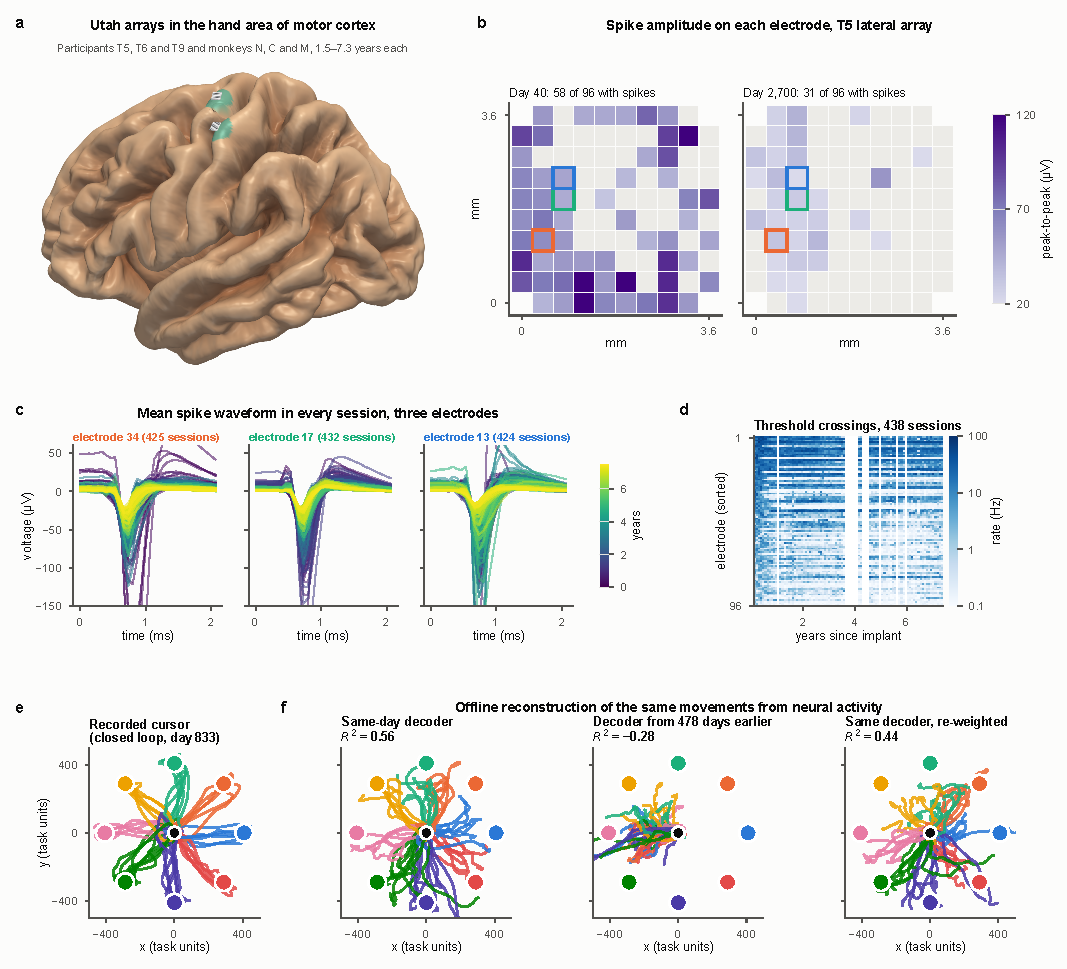
\includegraphics[width=170mm]{fig1_overview.pdf}}
\caption{\textbf{Recordings change over years, and decoders decay with them.} \textbf{a}, Approximate array sites
on the hand area of motor cortex, rendered on the FreeSurfer fsaverage cortical surface. \textbf{b}, Peak-to-peak spike
amplitude on each electrode of T5's lateral array, 7.3 years apart. Grey cells had no spikes. Outlines mark the
electrodes in \textbf{c}. \textbf{c}, Mean spike waveform of three electrodes in every session with spikes, coloured
by time since implant. \textbf{d}, Threshold-crossing rate of every electrode on the same array in every session, in
30-day bins. White columns have no sessions. \textbf{e}, Recorded cursor paths in a closed-loop session of T5, for
held-out outward movements. Colours mark targets. \textbf{f}, The same movements reconstructed offline from neural
activity by three decoders. The decoder from day 355 fails without correction and recovers after re-weighting each
channel (Methods).}
\label{fig:overview}
\end{figure}

\section*{Results}

\subsection*{Datasets and approach}

We assembled four public datasets (Fig.~\ref{fig:design}a and Supplementary Table~1). Decoder analyses used six
individuals. Monkey N was recorded over 1,242 days with Utah arrays in motor cortex during a two-finger
task\cite{temmar2025,nason2021}. Monkeys C and M were recorded over three and 1.5 years during
reaching\cite{gallego2020,perich2018}. BrainGate participants T6, T5 and T9 contributed 124, 92 and 117 closed-loop
cursor sessions over 3.1, 7.2 and 2.0 years\cite{hahn2026}. Electrode analyses used all 20 arrays from 14 BrainGate
participants (2,289 sessions) and monkey N. Monitoring analyses used closed-loop sessions in which participants T11
and T5 controlled a cursor with a fixed decoder\cite{pun2024}.

For each individual, we trained a linear decoder on one session and tested it on later sessions at gaps of 1 to 480
days. Before testing, every channel of the later session was z-scored with that session's own mean and standard
deviation. This step, renormalization, needs no labels and equalizes each channel's scale; the result is the
renormalized fixed decoder. We then applied a ladder of corrections (Fig.~\ref{fig:design}b and Methods). Label-free
corrections updated channel means or aligned neural activity to the training day. Corrections that use labeled trials
from the later day either re-weighted each channel's contribution to the otherwise unchanged decoder, or refitted the
decoder while shrinking it toward the old one. A decoder trained on the later day served as the reference. We report
retention, the ratio of a decoder's accuracy (coefficient of determination, $R^2$) to that of the reference on the same
test trials.

\begin{figure}[tbp]
\centering
\makebox[\textwidth][c]{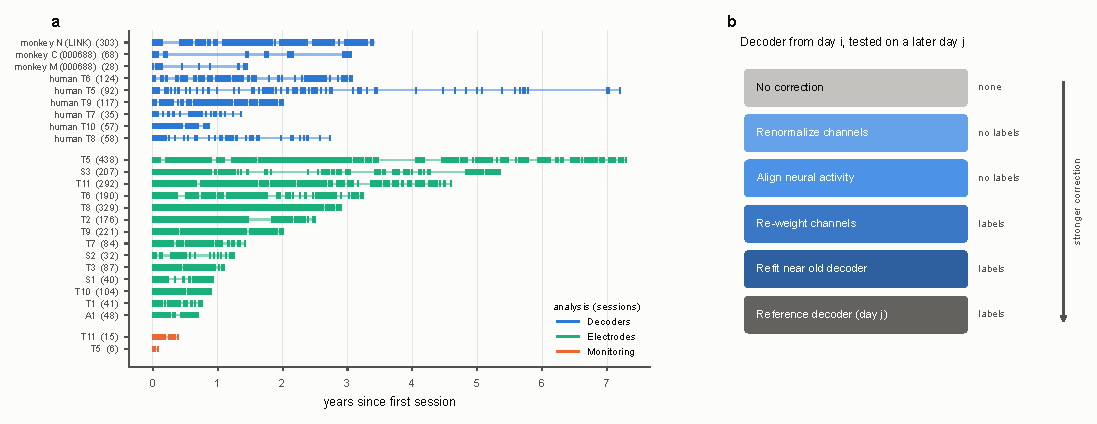
\includegraphics[width=170mm]{fig2_design.pdf}}
\caption{\textbf{Datasets and the correction ladder.} \textbf{a}, Sessions analyzed, by individual. Each tick is one
session. Numbers give sessions per analysis. \textbf{b}, The correction ladder. A decoder trained on day $i$ is tested on
a later day $j$ after increasingly strong corrections. A decoder trained on day $j$ is the reference.}
\label{fig:design}
\end{figure}

\subsection*{Decay rates differ about a hundredfold between individuals}

Without any correction, decoders failed: reusing the training day's normalization gave median $R^2$ below zero at most
gaps (Supplementary Table~2). We therefore use the renormalized fixed decoder as the baseline.

How much accuracy survived a single night differed between individuals (Fig.~\ref{fig:decay}a,b). For one-day gaps,
retention was \val{N:strict1} in monkey N (95\% confidence interval \val{N:strict1ci}; $n = \val{N:strict1n}$ pairs),
\val{C:strict1} in monkey C (\val{C:strict1ci}; $n = \val{C:strict1n}$), \val{M:strict1} in monkey M (\val{M:strict1ci};
$n = \val{M:strict1n}$) and \val{T9:strict1} in participant T9 (\val{T9:strict1ci}; $n = \val{T9:strict1n}$). One-day
pairs were rare in T6 ($n = \val{T6:strict1n}$) and T5 ($n = \val{T5:strict1n}$); at two days, retention was
\val{T6:strict2} in T6 ($n = \val{T6:strict2n}$) and \val{T5:strict2} in T5 ($n = \val{T5:strict2n}$).

Longer-term decay differed far more. Retention fell to one half within \val{T9:thalf} days in T9 (95\% confidence
interval \val{T9:thalfci}), \val{T5:thalf} days in T5 (\val{T5:thalfci}), \val{N:thalf} days in monkey N (\val{N:thalfci})
and \val{C:thalf} days in monkey C (\val{C:thalfci}). It took \val{M:thalf} days in monkey M (\val{M:thalfci}) and
\val{T6:thalf} days in T6 (\val{T6:thalfci}; Fig.~\ref{fig:decay}a,c). In monkey N and the three participants, the
reference decoder was equally accurate at short and long gaps (Supplementary Table~2). The decline therefore reflects a
growing mismatch between decoder and day, not poorer recordings.

\begin{figure}[tbp]
\centering
\makebox[\textwidth][c]{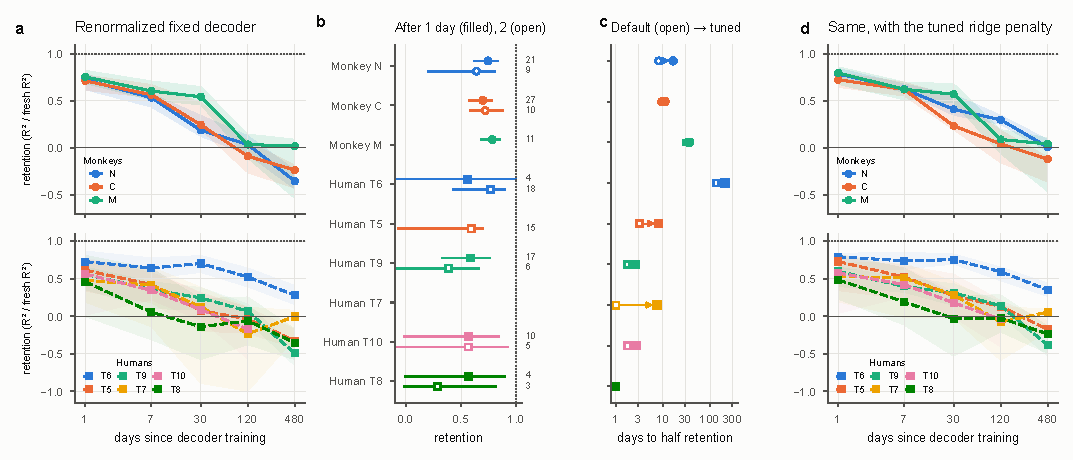
\includegraphics[width=170mm]{fig3_decay.pdf}}
\caption{\textbf{Decoders decay at rates that differ between individuals.} \textbf{a}, Retention of the renormalized fixed
decoder, the $R^2$ of the old decoder divided by that of the reference decoder, against days since training. Circles,
monkeys; squares, humans. Bands show 95\% confidence intervals. \textbf{b}, Retention after exactly one day (filled) and
two days (open). Numbers give session pairs. \textbf{c}, Days until retention falls to one half, with the default ridge
penalty (open) and the tuned penalty (filled). \textbf{d}, As in \textbf{a}, with the tuned penalty.}
\label{fig:decay}
\end{figure}

\subsection*{Weak regularization exaggerates decay}

Part of the measured decay came from the decoder rather than the recordings. We had adopted the ridge penalty used in
the original monkey N study\cite{temmar2025} ($\alpha = 0.1$; $\alpha = 1$ for the sparser spike counts of monkeys C and
M). With a stronger penalty ($\alpha = 10^4$), the time to half retention roughly doubled in three individuals: monkey N
(\val{N:thalf} to \val{N:thalftuned} days), T6 (\val{T6:thalf} to \val{T6:thalftuned} days) and T5 (\val{T5:thalf} to
\val{T5:thalftuned} days). It changed little in monkeys C and M and in T9 (Fig.~\ref{fig:decay}c,d). Per training session, absolute $R^2$ on
later days rose by a median of \val{N:tunedabsdiff} in monkey N (two-sided Wilcoxon signed-rank test,
$P = \val{N:tunedabsp}$) and \val{T6:tunedabsdiff} in T6 ($P = \val{T6:tunedabsp}$). Reports of decoder decay therefore
depend on how strongly the decoder was regularized, and we use the tuned penalty for the remaining decoder analyses
unless stated.

\subsection*{Per-channel rescaling outperforms label-free alignment}

Several methods realign neural activity to a reference day without labels\cite{degenhart2020,gallego2020,
farshchian2019,ma2023,karpowicz2025}. Their benefits were usually measured against a fixed decoder or against one whose
channel means alone were updated\cite{ma2023,wilson2025}. We compared such corrections with renormalization
(Fig.~\ref{fig:labelfree}a and Supplementary Table~3).

Updating channel means alone was worse than renormalization in every individual; in monkey N the difference was
\val{N:renmeandiff} in $R^2$ (two-sided Wilcoxon signed-rank test over training sessions, $P = \val{N:renmeanp}$).
Rotating the dominant neural subspace onto the training day by orthogonal Procrustes analysis\cite{schonemann1966} did
not close this gap. Applied after updating means, it lowered $R^2$ further in monkey N (by \val{N:rotmeandiff};
$P = \val{N:rotmeanp}$). Applied after renormalization, it lowered $R^2$ slightly in every individual, for example by
\val{N:rotrendiff} in monkey N ($P = \val{N:rotrenp}$). Matching the full channel covariance (CORAL\cite{sun2016})
improved slightly on renormalization in monkey N (by \val{N:coraldiff}; $P = \val{N:coralp}$), did not differ in monkeys
C and M, and was worse in the three participants. A faithful implementation of the factor-analysis stabilizer of
Degenhart and colleagues\cite{degenhart2020} was better than renormalization in T5 (by \val{T5:stabrendiff};
$P = \val{T5:stabrenp}$), did not differ in monkey N and was worse in the other four individuals. That method was
designed for closed-loop use with a latent decoder, and offline tests may understate it. Methods that align latent
dynamics with labeled data\cite{gallego2020} or adversarial networks\cite{farshchian2019,ma2023,karpowicz2025} were not
tested. Among the corrections we tested, however, the label-free step that mattered was rescaling each channel, and
gains reported for alignment over mean-only baselines\cite{wilson2025} may largely reflect this step.

\subsection*{Label-free monitoring adds little beyond elapsed time}

A monitor that warns when a decoder is failing could make recalibration less frequent. MINDFUL scores instability as
the divergence between distributions of neural features, or of decoder outputs, on a test day and a reference
day\cite{pun2024}. Such scores correlate with decoder error, but both grow with time since calibration.

Offline in monkey N (537 session pairs), elapsed time alone correlated with decoder accuracy (Spearman
$|\rho| = \val{mon:days}$; Fig.~\ref{fig:labelfree}b). Neural divergence correlated more weakly
($|\rho| = \val{mon:neuralraw}$), and its partial correlation fell to \val{mon:neuralpart} after controlling for elapsed
time; output divergence behaved the same way. Adding both divergences to elapsed time slightly increased the
cross-validated error of predicted $R^2$ (\val{mon:maeboth} versus \val{mon:maedays}). A pilot on the first year of monkey
N tested a broader set of label-free statistics, and none improved on elapsed time (Supplementary Note~1). This was not
because the remaining variation was noise: day-to-day performance beyond the time trend was reliable (split-half
reliability 0.84).

We then re-analyzed the public MINDFUL data, in which T11 and T5 controlled a cursor in closed loop with a fixed decoder
(Fig.~\ref{fig:labelfree}c and Supplementary Table~4). In T11 (\val{T11:mf:ndays} days), neural divergence correlated with
angular error across 60-s windows ($r = \val{T11:mf:nraw}$), consistent with the original report\cite{pun2024}. Most of
this association was shared with elapsed time (partial $r = \val{T11:mf:npart}$), and adding neural divergence did not
improve leave-one-day-out prediction of error (\val{T11:mf:dn}\textdegree{} versus \val{T11:mf:days}\textdegree{}).
Output divergence kept a partial correlation of \val{T11:mf:opart}, and adding it reduced the error to
\val{T11:mf:do}\textdegree. These window-level statistics are nested within few days, and output divergence and angular
error are both computed from the cursor's motion, so part of their link is mechanical. The six days available for T5
allow only a descriptive comparison. Within these limits, elapsed time was as good a guide as neural statistics.

\begin{figure}[tbp]
\centering
\makebox[\textwidth][c]{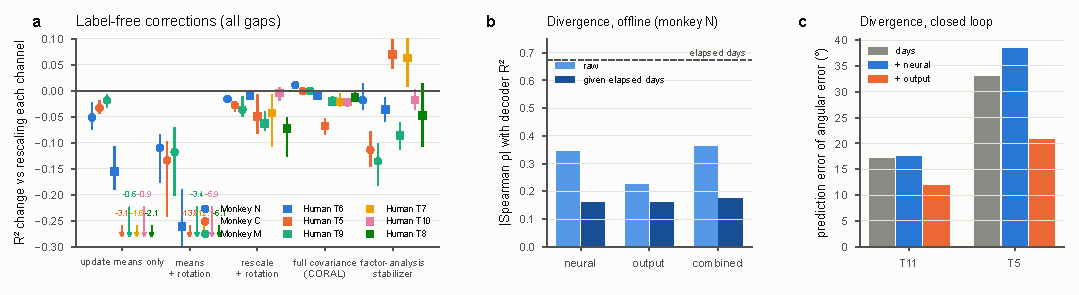
\includegraphics[width=170mm]{fig4_labelfree.pdf}}
\caption{\textbf{Label-free corrections and monitoring add little.} \textbf{a}, Change in $R^2$ for five label-free
corrections, relative to renormalization. Points show medians over training sessions; bars show 95\% confidence
intervals. Values below the axis are printed. \textbf{b}, Offline monitoring in monkey N. Bars show how strongly each
divergence score correlates with decoder accuracy, before (light) and after (dark) removing the effect of elapsed time.
The dashed line marks elapsed time alone. \textbf{c}, Closed-loop monitoring in the public MINDFUL data. Bars show the
error in predicting cursor angular error from elapsed days alone, or with a divergence score added.}
\label{fig:labelfree}
\end{figure}

\subsection*{Channel tuning is partly preserved over months}

Label-free corrections left much of the loss in place. We next asked what kind of change the remaining loss reflects.
For this we used re-weighting: one weight per channel in front of the otherwise unchanged decoder, fitted with labeled
trials from the later day. Re-weighting lets each channel's contribution grow, shrink or vanish, but keeps the decoder's pattern
across time lags and outputs. In the three participants it restored retention to \val{T9:tgainretmin}--\val{T6:tgainretmax}
at every gap up to 480 days, recovering \val{T6:trecmin}--\val{T6:trecmax}\%, \val{T5:trecmin}--\val{T5:trecmax}\% and
\val{T9:trecmin}--\val{T9:trecmax}\% of the loss in T6, T5 and T9 (Fig.~\ref{fig:channels}a). In the monkeys it recovered
\val{N:trecmin}--\val{N:trecmax}\%, \val{C:trecmin}--\val{C:trecmax}\% and \val{M:trecmin}--\val{M:trecmax}\%.

This difference between species mostly reflects what was decoded, not how the recordings changed. A two-dimensional
target, such as the cursor-to-target direction decoded for the participants, can be fitted from many channel weights even
when the decoder's per-channel patterns are wrong. To test this, we re-weighted decoders whose channels had been randomly
scrambled (Fig.~\ref{fig:channels}b and Supplementary Table~5). In T5, the scrambled decoder reached a retention of
\val{T5:ctl:rew_perm}, close to the \val{T5:ctl:rew} of the correctly assigned decoder; in T9 the values were
\val{T9:ctl:rew_perm} and \val{T9:ctl:rew}. In the monkeys, whose decoders predicted four kinematic signals, scrambled
decoders could not be rescued (retention \val{N:ctl:rew_perm}, \val{C:ctl:rew_perm} and \val{M:ctl:rew_perm}). Decoding
hand-movement direction in monkeys C and M raised the share of the loss recovered to \val{C:matchrecmin}--\val{C:matchrecmax}\%
and \val{M:matchrecmin}--\val{M:matchrecmax}\% (Supplementary Table~7), but did not reproduce the human setting.

Channel identity nevertheless mattered in every individual. Correctly assigned decoders always beat scrambled ones, and
the difference was largest when weights could not change sign, so that scrambled channels could not be reversed. With
non-negative weights, retention was \val{T6:ctl:rew_nonneg} versus \val{T6:ctl:rew_perm_nn} in T6,
\val{T5:ctl:rew_nonneg} versus \val{T5:ctl:rew_perm_nn} in T5 and \val{T9:ctl:rew_nonneg} versus \val{T9:ctl:rew_perm_nn}
in T9, and \val{N:ctl:rew_nonneg} versus \val{N:ctl:rew_perm_nn}, \val{C:ctl:rew_nonneg} versus \val{C:ctl:rew_perm_nn}
and \val{M:ctl:rew_nonneg} versus \val{M:ctl:rew_perm_nn} in the monkeys. Constraining the weights to be non-negative
cost little with correct channels. Drift therefore preserves much of each channel's tuning pattern.

The per-channel weights also related to measured changes at each electrode (Fig.~\ref{fig:channels}c and Supplementary
Table~5). For each pair, we compared the fitted weights with the change in each electrode's threshold-crossing rate
between the two days, recorded independently in the BrainGate yield data. Channels whose spiking rose received larger
weights in all three participants. The median Spearman correlation per training session was \val{T6:mech:rate:rho} in
T6 (positive in \val{T6:mech:rate:pos}\% of sessions; two-sided Wilcoxon signed-rank test, $P = \val{T6:mech:rate:p}$),
\val{T5:mech:rate:rho} in T5 (\val{T5:mech:rate:pos}\%; $P = \val{T5:mech:rate:p}$) and \val{T9:mech:rate:rho} in T9
(\val{T9:mech:rate:pos}\%; $P = \val{T9:mech:rate:p}$), against near zero after shuffling channels. In T9, channels whose
impedance rose received smaller weights (median correlation \val{T9:mech:imp:rho}; $P = \val{T9:mech:imp:p}$). These
relations are weak for single channels but consistent, linking the decoder's corrections to physical changes at the
array.

The results held for nonlinear decoders. We trained a recurrent network decoder, regularized so that it could not
memorize the closed-loop sessions (Methods). It was slightly less accurate than the linear decoder in people (median $R^2$ \val{T6:nnown},
\val{T5:nnown} and \val{T9:nnown} versus \val{T6:linown}, \val{T5:linown} and \val{T9:linown}) and more accurate in
monkeys. Re-weighting its input channels recovered \val{T6:nnrecmin}--\val{T6:nnrecmax}\%,
\val{T5:nnrecmin}--\val{T5:nnrecmax}\% and \val{T9:nnrecmin}--\val{T9:nnrecmax}\% of its loss in the participants and
\val{N:nnrecmin}--\val{N:nnrecmax}\%, \val{C:nnrecmin}--\val{C:nnrecmax}\% and \val{M:nnrecmin}--\val{M:nnrecmax}\% in the
monkeys (Fig.~\ref{fig:channels}d and Supplementary Table~6). Finally, we measured the angle between decoders fitted on different days. Allowing one scale per channel reduced this
angle by \val{ang:redmin}--\val{ang:redmax}\textdegree{} in every individual (Supplementary Table~8). Angles that allow
only a global scale therefore overstate how much decoders rotate across days\cite{wilson2025}.

\begin{figure}[tbp]
\centering
\makebox[\textwidth][c]{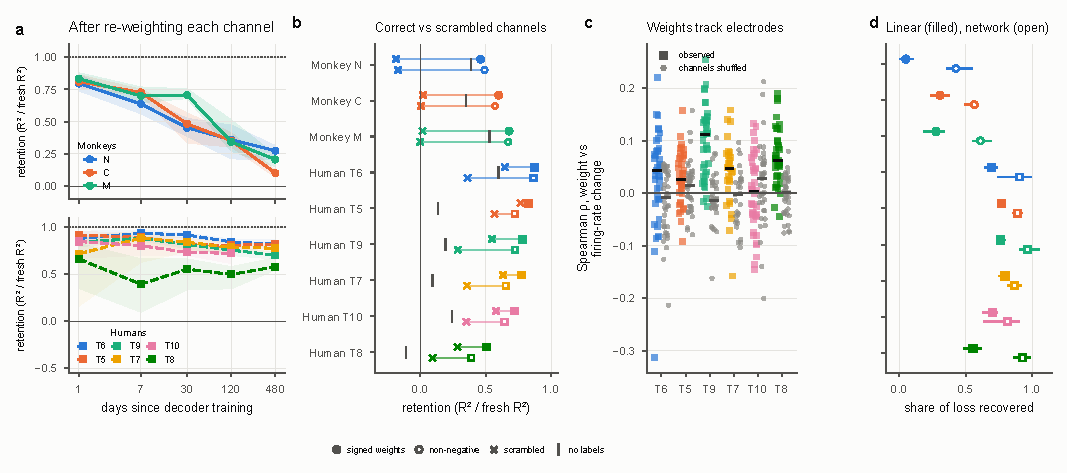
\includegraphics[width=170mm]{fig5_channels.pdf}}
\caption{\textbf{Channel tuning is partly preserved over months.} \textbf{a}, Retention after re-weighting each channel in
front of the unchanged decoder. \textbf{b}, Retention after re-weighting the correct decoder (circles and squares) or a
decoder with scrambled channels (crosses). Upper rows use signed weights; lower rows use non-negative weights. Ticks mark
the renormalized fixed decoder. \textbf{c}, Correlation between the fitted channel weights and each electrode's change in
firing rate. Each point is one training session. Grey points show the same after shuffling channels. \textbf{d}, Share of
the lost accuracy recovered by re-weighting, for linear (filled) and recurrent (open) decoders. Bars show 95\%
confidence intervals.}
\label{fig:channels}
\end{figure}

\subsection*{A few minutes of labeled data restore decoders in people}

How much labeled data does recalibration need? In the three participants, retention pooled over all gaps rose from
\val{hum:effnone} without labels to \val{hum:effL6n50} with 50 labeled trials and \val{hum:effL6n100} with 100 for a
freshly trained, strongly regularized decoder (Fig.~\ref{fig:recipes}c and Supplementary Table~10). Refitting while
shrinking toward the old decoder reached \val{hum:effL6pn50} and \val{hum:effL6pn100}, and re-weighting reached
\val{hum:effL3n50} and \val{hum:effL3n100}. Movement periods lasted 1.6--3.9~s in these sessions, so 100 trials take a few
minutes. Recovery was slower in T9 than in T5 and T6 (Supplementary Table~10). Re-weighting therefore indicates what
changes, but it is not the most data-efficient recalibration in these sessions.

Two further choices made recalibration more reliable. First, the ridge penalty can be tuned on training-day data alone.
We chose the largest penalty whose same-day accuracy stayed within 1\% of the best. This rule raised cross-day $R^2$ in
every individual without lowering same-day accuracy (Fig.~\ref{fig:recipes}a,b and Supplementary Table~9). Session-level
median gains were \val{N:rulemed} in monkey N ($P = \val{N:rulep}$) and \val{T6:rulemed}, \val{T5:rulemed} and
\val{T9:rulemed} in the participants. Ordinary same-day tuning usually chose a similar penalty (Methods).
Second, with very few trials, refitting can make a decoder worse. In monkey N (86 session pairs), choosing the shrinkage
strength by cross-validation on 10 trials made \val{harm:10:cv}\% of recalibrations worse than no recalibration
(Fig.~\ref{fig:recipes}d). A fixed strong shrinkage, the value that worked best on other training sessions, lowered this
to \val{harm:10:hist}\% (exact McNemar test, $P = \val{mcn:10:p}$; Holm-adjusted over five data budgets,
$P = \val{mcn:10:holm}$); with 20 trials the rates were \val{harm:20:cv}\% and \val{harm:20:hist}\%
($P = \val{mcn:20:p}$; adjusted $P = \val{mcn:20:holm}$).

\begin{figure}[tbp]
\centering
\makebox[\textwidth][c]{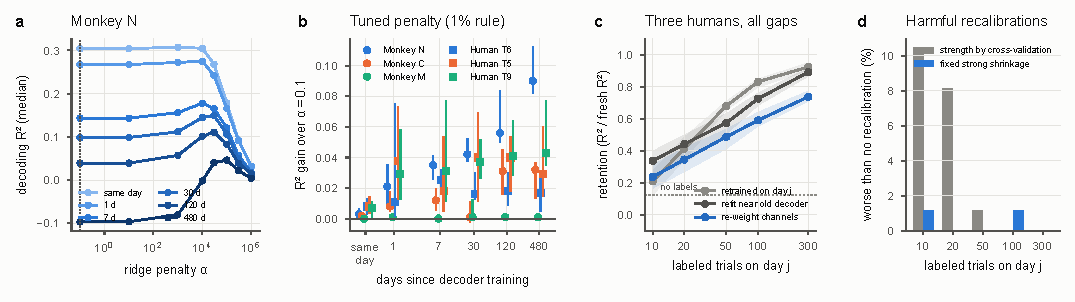
\includegraphics[width=170mm]{fig6_recipes.pdf}}
\caption{\textbf{Simple recipes for recalibration.} \textbf{a}, Decoding $R^2$ in monkey N against the ridge penalty, on the
training day (lightest) and on later days (darker). The dotted line marks $\alpha = 0.1$. \textbf{b}, Gain from the 1\%
rule over $\alpha = 0.1$, per individual and gap. \textbf{c}, Retention in the three participants against the number of
labeled trials, for a retrained decoder, a refit shrunk toward the old decoder and re-weighting. The dotted line marks
the renormalized fixed decoder. \textbf{d}, Recalibrations in monkey N that made the decoder worse than no recalibration,
with the shrinkage chosen by cross-validation (grey) or fixed (blue).}
\label{fig:recipes}
\end{figure}

\subsection*{Most electrode silences are transient fluctuations}

We next asked how single electrodes change over years. The BrainGate yield data report threshold-crossing rates and
impedance for every electrode in every session\cite{hahn2026}, and monkey N provides matching data. An
electrode was active when its threshold-crossing rate exceeded 2~Hz, the definition used by BrainGate\cite{hahn2026}.
Array yield and impedance declined over years in both species (Fig.~\ref{fig:electrodes}a,b). Impedance fell in 17 of
18 human arrays with measurements (median Spearman $\rho$ with time $-0.92$). In monkey N it fell from a median of
302~k$\Omega$ in the first year to 171~k$\Omega$ in the fourth ($\rho = -0.88$). Both trends replicate earlier
reports\cite{barrese2013,sponheim2021,chen2023,bjanes2025,hahn2026}.

Electrodes often fell silent and later recovered\cite{barrese2013,downey2018}, but most such events were fluctuation
(Fig.~\ref{fig:electrodes}c and Supplementary Table~11). Of \val{null:base:sil} initially active human electrodes that
stayed below threshold for at least three consecutive sessions, \val{null:base:obs}\% later recovered for at least three
sessions. When each electrode's session order was shuffled 200 times, which destroys any temporal process, the recovery
rate was \val{null:base:mean}\% (95\% range \val{null:base:ci}\%; permutation $P = \val{null:base:p}$). The match also held
when silence required rates below 0.5~Hz, and with a fixed threshold in microvolts for each electrode, which prevents
changes in noise level from moving the threshold. Silences lasting at least 30 days were different. They were twice as common as in the
shuffled data (\val{null:long_silence:sil} versus \val{null:long_silence:silnull} on average), and \val{null:long_silence:obs}\% of
them ended in recovery, against \val{null:long_silence:mean}\% in the shuffled data (95\% range \val{null:long_silence:ci}\%;
$P = \val{null:long_silence:p}$). Recovery here means that the electrode again recorded spiking, not necessarily from the
same neuron.

Spiking declined somewhat faster at the edge of the array than in its interior (Fig.~\ref{fig:electrodes}d). Among
initially active electrodes, the edge decline was steeper in \val{edge:raw:neg} of \val{edge:raw:n} human arrays with at
least 10 such electrodes (Wilcoxon signed-rank test with the array as the unit, one-sided $P = \val{edge:raw:wil}$).
After adjusting for each electrode's initial firing rate, the effect weakened (\val{edge:adj:neg} of \val{edge:adj:n}
arrays; one-sided $P = \val{edge:adj:wil}$). In monkey N, edge electrodes declined faster within both arrays for
threshold crossings but not for spike-band power. These trends agree with models in which micromotion strains tissue
most at the array edges\cite{forrest2025}, but they are modest and partly explained by initial activity.

\begin{figure}[tbp]
\centering
\makebox[\textwidth][c]{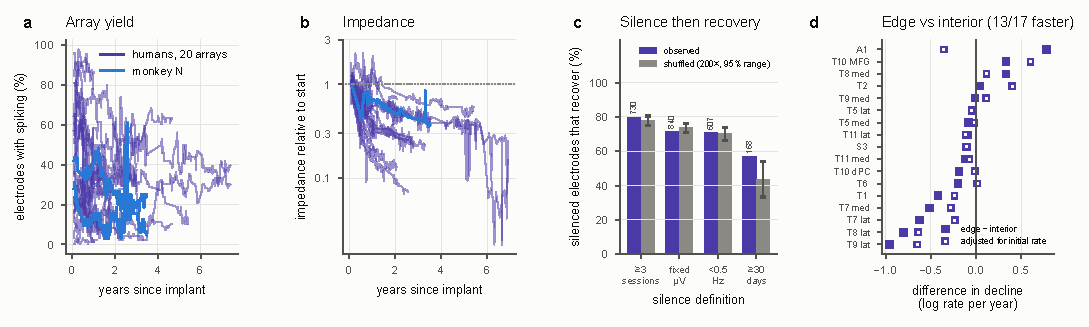
\includegraphics[width=170mm]{fig7_electrodes.pdf}}
\caption{\textbf{Most electrode silences are transient fluctuations.} \textbf{a}, Percentage of electrodes with spiking
activity over years, for 20 human arrays (purple) and two arrays in monkey N (blue). \textbf{b}, Median impedance of each
array relative to its first sessions. \textbf{c}, Percentage of silenced human electrodes that later recovered, observed
(purple) and after shuffling session order 200 times (grey, with 95\% range). Four definitions of silence are shown.
Numbers give silenced electrodes. \textbf{d}, Difference in the yearly decline of firing rate between edge and interior
electrodes, per human array, before (filled) and after (open) adjusting for initial firing rate.}
\label{fig:electrodes}
\end{figure}

\subsection*{A calibrated simulator for testing new corrections}

Methods for stable decoding are hard to compare without a common test bed\cite{karpowicz2024falcon}. We built a
feature-level simulator that takes a real session and returns it as it might appear days to years later (Methods). It
combines mixing of signals between channels, gradual turnover of each channel's tuning and switching of electrodes
between active and silent states. Switching rates came from monkey N's electrode statistics. The mixing and turnover
parameters were calibrated so that the simulated correction ladder matched monkey N's during its first 700 days. The
fit had a root-mean-square error of \val{sim:rms} in retention (Fig.~\ref{fig:sim}a).

We tested the simulator on the later days, which it had not seen, against two baselines (Fig.~\ref{fig:sim}b). A
simulator without drift was far worse (median absolute error \val{sim:unfit:nodrift}--\val{sim:budget:nodrift}). A
stronger baseline simply reused the median retention measured in the first 700 days. This empirical curve was as good as
or better than the simulator for the corrections used in calibration and for different amounts of labeled data (\val{sim:fit:early} versus \val{sim:fit:sim}, and \val{sim:budget:early} versus \val{sim:budget:sim}). For
corrections that the simulator was not fitted to, it was clearly better (\val{sim:unfit:sim} versus
\val{sim:unfit:early}). The simulator is therefore most useful for predicting how new corrections will behave. Real
decoders decayed more slowly in the later years. A calibration on that period gave weaker session-to-session mixing
(\val{sim:mix0late} versus \val{sim:mix0}) and slower turnover (time constant \val{sim:taurholate} versus \val{sim:taurho}
days; Fig.~\ref{fig:sim}c and Supplementary Table~12). Drift may therefore slow as an implant ages, at least in this
monkey.
Training decoders on simulated futures helped little ($R^2$ higher by \val{aug:sim}) compared with stronger
regularization (\val{aug:ridge_reg}) or training on several past sessions (\val{aug:multi}; Supplementary Table~13).

\begin{figure}[tbp]
\centering
\makebox[\textwidth][c]{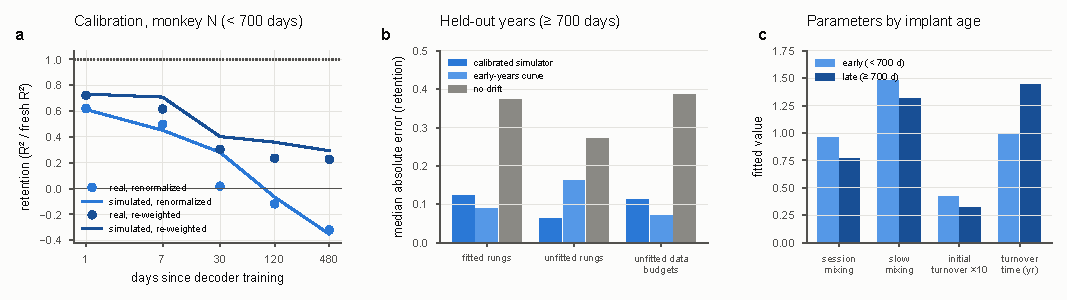
\includegraphics[width=170mm]{fig8_simulator.pdf}}
\caption{\textbf{A calibrated simulator for testing new corrections.} \textbf{a}, Calibration on monkey N sessions before
day 700. Points show real retention; lines show the simulator. \textbf{b}, Prediction error on sessions after day 700,
for the simulator (dark blue), the median retention measured before day 700 (light blue) and a simulator without drift
(grey). \textbf{c}, Parameters calibrated separately on early and late sessions.}
\label{fig:sim}
\end{figure}

\section*{Discussion}

We measured how intracortical BCIs age, at the level of decoders and of electrodes, in three monkeys and 14 people with
one pipeline. Five findings stand out. Decay rates differ about a hundredfold between individuals. Measured decay
depends on how strongly the decoder is regularized. In people, a few minutes of labeled data restore most of the
accuracy, whereas the label-free corrections we tested add little beyond rescaling each channel. Corrections work far
better when each channel keeps its identity, and they track changes at each electrode. And most brief electrode
silences are noise, while long ones are real and often reverse.

These findings have direct implications for building durable interfaces. Because decay rates vary so widely, a fixed
recalibration schedule is unlikely to suit all users, and schedules may need to be set per person. Because weak
regularization exaggerates decay, comparisons of decoder longevity are meaningful only between well-regularized
decoders. Per-channel renormalization is the appropriate baseline for evaluating label-free methods; earlier
comparisons against fixed or mean-only decoders\cite{ma2023,wilson2025} probably overstated their benefit. For
recalibration in people, any well-regularized refit with about 100 labeled trials recovered most of the accuracy in our
data. When only a few trials are available, shrinking toward the previous decoder, including its intercept, prevents
harmful updates. These are simple, inexpensive steps, and they set the bar that more sophisticated methods should
clear.

The channel analyses clarify what changes. Earlier work modeled per-electrode drift as shifts in baseline over
weeks\cite{bishop2014,jarosiewicz2015}, and human decoders absorb day-to-day changes with input layers learned for each
day\cite{willett2021,fan2023}. Other studies describe changes in the preferred directions of individual
features\cite{pun2024} and rotation of decoder weights\cite{wilson2025}. In our data, much of each channel's tuning
pattern survived for months: decoders with correctly assigned channels consistently beat scrambled ones, and the
per-channel corrections tracked each electrode's firing. At the same time, our scrambled-channel control shows that high
recovery from a per-channel correction is not, by itself, evidence of per-channel drift when the decoded variable is
low-dimensional. Correction-based analyses of drift, including ours, need such controls. Changes in the number or
proximity of neurons near each electrode would produce per-channel changes\cite{polikov2005,kozai2015}, but our data
cannot identify the cause.

The electrode analyses refine common descriptions of array decline. Activity near the yield threshold fluctuated
strongly between sessions, and most short silences were no more than that. Yield counts from single sessions are
therefore noisy, and channels that fall silent for a few sessions are likely to return. Silences lasting over a month
were real and still reversed in more than half of cases. Hahn and colleagues analyzed yield, decoding signal quality and
tuning stability in the same human data\cite{hahn2026}. We add three analyses: silence and recovery tested against a
permutation null, edge-biased spiking loss tested with the array as the unit, and a link between electrode changes and
decoder corrections.

Our study has limitations. All analyses were offline; offline variability can overstate online decay\cite{flint2013},
and in closed loop users adapt to their decoder\cite{gilja2012}. Human decoding labels were inferred from the direction
from cursor to target, and the online decoder shaped both the neural activity and the cursor path. Three participants and
three monkeys cannot establish population rates, and the datasets differ in task, signal type, array placement and
implant age. The label-free comparisons covered three classes of method and did not include latent-dynamics or
adversarial alignment. The simulator is calibrated to feature-level statistics in one monkey and does not model
biophysics.

Long-term public datasets made this study possible. We release our code, derived results and the calibrated simulator
so that others can test methods against realistic drift. Our results suggest that keeping implanted decoders working
over months depends less on elaborate corrections than on well-regularized decoders, proper per-channel normalization
and short, careful recalibration.

\section*{Methods}

\subsection*{Datasets and ethics}

All data were public and de-identified. The original studies obtained ethical approval and informed consent, as
described in the cited publications. We collected no new data.

\textit{Monkey N} (LINK; DANDI Archive 001201\cite{data_link}; ref.~\cite{temmar2025}). One rhesus macaque had Utah arrays
in the hand area of primary motor cortex\cite{nason2021}. The release contains 312 sessions on 303 days over 1,242 days,
in which the monkey moved two finger groups to targets in center-out or random-target blocks. We used the 96 released
channels (64 on the medial array and 32 on the lateral array), with spike-band power and threshold crossings at $-4.5$
times the root-mean-square noise in 20~ms bins\cite{nason2020}. Outputs were the position and velocity of the two finger
groups. Electrode impedance was stored on 228 days.

\textit{Monkeys C and M} (DANDI Archive 000688\cite{data_perich}; refs.~\cite{gallego2020,perich2018}). Both monkeys had
Utah arrays in motor and premotor cortex and performed center-out and random-target reaching. Monkey C had 68 sessions
from October 2013 to October 2016, and monkey M had 28 sessions from January 2014 to June 2015. We summed the spikes of
all sorted units on each electrode in 20~ms bins, giving 96 (C) or 192 (M) channels. Hand position and velocity were
interpolated to bin centers.

\textit{BrainGate participants} (Dryad\cite{data_braingate}; ref.~\cite{hahn2026}). The yield data contain one recording
from each of 2,289 research sessions in 14 participants with 20 arrays (A1, S1--S3, T1--T3 and T5--T11). For every
electrode, they list threshold-crossing rates at several thresholds (with the threshold in microvolts), impedance and
grid position. Nineteen arrays were in the hand area of motor cortex and one was in the middle frontal gyrus. The
decoding data contain closed-loop cursor sessions with spike-band power in 10~ms bins, cursor and target positions and
the periods of attempted movement. We used all sessions of T6 (124 sessions over 3.1 years, one array, 96 channels), T5
(92 sessions over 7.2 years, two arrays, 192 channels) and T9 (117 sessions over 2.0 years, two arrays, 192 channels).
Sessions contained a median of 367, 551 and 275 trials, with median movement periods of 1.6, 1.7 and 3.9~s. All sessions
of a participant were treated as one task type.

\textit{MINDFUL} (Dryad\cite{data_mindful}; ref.~\cite{pun2024}). Closed-loop cursor blocks in which T11 (15 days) and T5
(6 days) used a fixed decoder, with neural features in 20~ms bins (spike-band power for T11 and threshold crossings for
T5), the decoder's velocity output and the angular error of the cursor.

\subsection*{Features, decoders and accuracy}

For monkey N and the human participants we used spike-band power (human 10~ms bins averaged in pairs). For monkeys C and
M we used per-electrode spike counts. Each channel was z-scored with the mean and standard deviation of the decoding
session's training segment, computed without labels (renormalization). The linear decoder was ridge
regression\cite{hoerl1970} on 8 causal lags (160~ms) of the z-scored features, with an unpenalized intercept. The default
penalty was $\alpha = 0.1$ for monkey N and the humans, adopted from ref.~\cite{temmar2025}, and $\alpha = 1$ for monkeys C
and M; the tuned penalty was $\alpha = 10^4$ for the decoder trained on day $i$ and for the reference decoder. Outputs were
finger position and velocity for monkey N, hand position and velocity for monkeys C and M, and for the humans the
intended movement direction, defined as the unit vector from cursor to target during attempted movement. Accuracy was
the coefficient of determination $R^2$, averaged over outputs and computed on held-out trials of the test session. In
monkey N the first 300 of 375 trials trained the decoder, as in ref.~\cite{temmar2025}; in the other datasets the first
80\% of trials did.

The recurrent decoder was a long short-term memory network\cite{hochreiter1997} with 64 hidden units, input
dropout\cite{srivastava2014} of 0.5 and 20-bin input windows (400~ms). It was trained with AdamW\cite{loshchilov2019}
(learning rate $10^{-3}$, weight decay 0.01) for up to 4,000 iterations of 256 samples, with early stopping on the last
20\% of training trials checked every 100 iterations. Without these measures, a 256-unit network memorized the human
training sessions (training $R^2$ 0.97, test $R^2$ $-1.1$ on one session). The network analyses used 25 training
sessions per individual chosen at random with a fixed seed.

\subsection*{Session pairs}

For each training session $i$ and target gap $g \in \{1, 7, 30, 120, 480\}$ days, we selected the later session $j$ of
the same task type whose gap was closest to $g$, within 25\% of $g$ or one day, whichever was larger. The one-day set
therefore contains one- and two-day gaps, which we report separately. In monkey N, 80 training sessions were drawn at
random with a fixed seed; the full monkey N set (537 pairs) also includes further gaps and was used for monitoring. Pair
counts are listed in Supplementary Table~2. The time to half retention was found by interpolating median retention at
the target gaps linearly in log days, with 95\% confidence intervals from a cluster bootstrap over training sessions.

\subsection*{Correction ladder}

Let $\mathbf{x}_j(t) \in \mathbb{R}^C$ be the raw features of test day $j$, $\boldsymbol{\mu}_d$ and
$\boldsymbol{\sigma}_d$ the channel means and standard deviations of day $d$, and $f_i$ the decoder trained on day $i$.

\begin{itemize}
\item \textit{No correction}: $f_i\big((\mathbf{x}_j - \boldsymbol{\mu}_i)/\boldsymbol{\sigma}_i\big)$.
\item \textit{Mean updating}: $f_i\big((\mathbf{x}_j - \boldsymbol{\mu}_j)/\boldsymbol{\sigma}_i\big)$.
\item \textit{Renormalization}: $f_i(\mathbf{z}_j)$ with $\mathbf{z}_j = (\mathbf{x}_j - \boldsymbol{\mu}_j)/
\boldsymbol{\sigma}_j$.
\item \textit{Re-weighting}: $f_i$ applied to $g_c z_{j,c}$ for each channel $c$, with one offset per output. The weights
$g_c$ (unconstrained in sign unless stated) were shrunk toward 1 and the offsets toward the old intercept; the penalty,
scaled by the number of samples, was chosen from $\{10^{-6}, \ldots, 10^2\}$ by five-fold cross-validation over contiguous
blocks of trials.
\item \textit{Ridge to prior}: a new decoder $(\mathbf{W}, \mathbf{b})$ fitted on the lagged features $\mathbf{H}$ of day
$j$ by minimizing
\begin{equation}
\|\mathbf{Y} - \mathbf{H}\mathbf{W} - \mathbf{1}\mathbf{b}^\top\|_F^2 + \lambda\left(\|\mathbf{W} - \mathbf{W}_i\|_F^2
+ \|\mathbf{b} - \mathbf{b}_i\|_2^2\right),
\label{eq:prior}
\end{equation}
where $(\mathbf{W}_i, \mathbf{b}_i)$ is the old decoder and $\lambda$ was chosen from $\{0.1, 1, \ldots, 10^6\}$ by
cross-validation.
\item \textit{Retrained decoder}: ridge regression on day $j$'s first $n$ labeled trials, with $\alpha$ chosen from the same
grid by cross-validation.
\item \textit{Reference}: a decoder trained on all of day $j$'s training trials.
\end{itemize}

\noindent Supervised rungs used the first $n$ labeled trials of day $j$ ($n = 300$, or all training trials if fewer,
unless stated). Retention was the ratio of a rung's $R^2$ to the reference $R^2$ on the same test trials, and the share
of the loss recovered by re-weighting was $(R^2_{\text{reweight}} - R^2_{\text{renorm}})/(R^2_{\text{ref}} -
R^2_{\text{renorm}})$. For the network decoder, re-weighting was a learned gain and offset per channel in front of the
frozen network, and the refit was fine-tuning with an $L_2$ penalty toward the old weights; penalties were chosen on the
last 20\% of labeled trials. We also computed a full input remap fitted by L-BFGS\cite{liu1989}; because it can represent
any linear decoder of the same form, we used it only as a calibration target for the simulator.

\textit{Channel controls.} For 40 training sessions per individual (fixed seed), re-weighting was repeated with weights
constrained to be non-negative (bounded least squares with the cross-validated penalty), and for a copy of the day-$i$
decoder whose channel weights were randomly permuted, with signed and with non-negative weights.

\textit{Electrode link.} For the same pairs in the human participants, the signed re-weighting weights were correlated
(Spearman) across channels with the change in log threshold-crossing rate ($\log(\text{rate} + 0.1)$ at $-4.5$ times the
noise) and in log impedance between the yield recordings of the two days, matched by electrode identity. A null
correlation was computed after permuting channels.

\textit{Matched-output control.} For monkeys C and M, sessions were rebuilt with a two-dimensional unit-vector target,
the direction of hand velocity, on bins where hand speed exceeded the session's 25th percentile, and the ladder was run on
the same pairs with the tuned penalty.

\textit{Decoder-weight angles.} Each channel's block of ridge weights (8 lags by all outputs) was stacked into
$\mathbf{B}_i$ and $\mathbf{B}_j$. We computed the angle between $\mathrm{vec}(\mathbf{B}_i)$ and $\mathrm{vec}(\mathbf{B}_j)$,
which allows one global scale, and the angle between $\mathrm{vec}(\mathbf{B}_j)$ and $\mathrm{vec}(\mathrm{diag}(\mathbf{s})
\mathbf{B}_i)$, with each channel's scale $s_c$ fitted by least squares.

\textit{Example in Fig.~\ref{fig:overview}.} Waveforms are the released robust mean waveforms (15~kHz, in microvolts)
for electrodes with a threshold-crossing rate of at least 2~Hz at $-4.5$ times the robust standard deviation. Amplitude is the
peak-to-peak value of these waveforms. Rates in panel d are the released threshold-crossing rates at the same
threshold, averaged within 30-day bins. The cortical surface was rendered with PyVista; array sites were placed
at the hand knob by MNI coordinates and are approximate. For the
reconstructions, decoders used the tuned penalty: one trained on T5's day 355, one trained on day 833, and the day-355
decoder re-weighted with 300 labeled trials from day 833. Paths are shown for held-out movements that started at the
center. Each path integrates the decoded direction from the cursor's start position. The step size was set so that
the intended direction would reach the target in the trial's duration, multiplied by a common display gain of 2 for
all decoders. $R^2$ values are those of the analysis on the same held-out trials.

\subsection*{Label-free corrections}

\textit{Procrustes rotation.} Let $\mathbf{V}_i, \mathbf{V}_j \in \mathbb{R}^{C\times k}$ hold the top $k = 16$ principal
axes of the corrected training features on each day. The orthogonal matrix $\mathbf{R}$ minimizing
$\|\mathbf{V}_j\mathbf{R} - \mathbf{V}_i\|_F$ was found by Procrustes analysis\cite{schonemann1966}, and inputs were mapped
as $(\mathbf{I} - \mathbf{V}_j\mathbf{V}_j^\top)\mathbf{z} + \mathbf{V}_i\mathbf{R}^\top\mathbf{V}_j^\top\mathbf{z}$. We
applied it to renormalized features and, separately, to mean-updated features with $\mathbf{V}_j$ estimated from those
features.

\textit{CORAL.} Renormalized day-$j$ features were re-colored to match day $i$'s covariance,
$\mathbf{z}' = \mathbf{C}_i^{1/2}\mathbf{C}_j^{-1/2}\mathbf{z}$\cite{sun2016}, with covariances shrunk 5\% toward a scaled
identity.

\textit{Factor-analysis stabilizer.} Following ref.~\cite{degenhart2020}, a factor-analysis model with 10 latent factors
was fitted to each day's renormalized training features, and a ridge decoder on 8 lags of the day-$i$ posterior latent
means was trained. On day $j$, a model fitted without labels was aligned to day $i$ by orthogonal Procrustes analysis of
the loadings of stable channels, found by iteratively keeping the 60\% of channels with the smallest loading residuals;
latents were then inferred from stable channels only and passed to the frozen latent decoder. The comparison baseline
reused the day-$i$ factor model on day $j$.

All label-free comparisons were summarized per training session over its pairs at all gaps.

\subsection*{Monitoring analyses}

In monkey N, for every pair we computed Gaussian Kullback--Leibler divergences between days $i$ and $j$ of the
projections of renormalized features on day $i$'s top ten principal axes (neural divergence) and of the decoder's
outputs (output divergence). We report raw Spearman correlations with $R^2$, partial correlations given log elapsed days
and time-blocked cross-validated linear prediction of $R^2$. The pilot statistics (first 46--61 sessions, 283 pairs) are
described in Supplementary Note~1; split-half reliability of the residual after the time trend used alternating pairs of
trials and the Spearman--Brown formula. For the MINDFUL data we followed the original definitions\cite{pun2024}:
non-overlapping 60~s windows, divergences against the first day, and the median angular error over non-excluded trials
(windows with fewer than 500 valid bins skipped). We report Pearson and partial correlations given elapsed days across
windows, and leave-one-day-out linear prediction of angular error; the reference day was excluded from evaluation.

\subsection*{Regularization and recalibration}

Ridge decoders were trained with $\alpha \in \{0.1, 10, 10^3, 10^4, 3\times10^4, 10^5, 3\times10^5, 10^6\}$ on 40
training sessions per individual (22 for monkey M) and evaluated on held-out same-day trials and on later sessions at
the five gaps. The 1\% rule chose the largest $\alpha$ whose median same-day $R^2$ was at least 99\% of the best median.
Compared with each training session's own best same-day penalty, the rule did not differ in monkeys C and M or in T6 and
added \val{N:rulevsbest} in monkey N ($P = \val{N:rulevsbestp}$), \val{T5:rulevsbest} in T5 and \val{T9:rulevsbest} in T9.
For the human data-efficiency analysis, the ladder was run for 30 training sessions per participant (fixed seed) with
$n \in \{10, 20, 50, 100, 300\}$. For harmful recalibrations we used 86 monkey N pairs with default-penalty decoders; the
shrinkage $\lambda$ in equation~(\ref{eq:prior}) was chosen per pair by cross-validation on the $n$ trials, or as the value
with the best median $R^2$ over pairs from other training sessions, which was $10^4$ for every pair with up to 50
trials. A recalibration was harmful when its $R^2$ was more than 0.01 below that of the renormalized fixed decoder.

\subsection*{Electrode statistics}

Statistics were computed per array. An electrode was active in a session when its threshold-crossing rate at $-4.5$ times
the root-mean-square noise was at least 2~Hz. An initially active electrode (mean rate of at least 2~Hz over the first
three sessions) was silenced at its first run of at least three consecutive observed sessions below threshold, and
recovered when it later exceeded 4~Hz for at least three consecutive sessions. Missing sessions were skipped, not
imputed. Control analyses (Supplementary Table~11) varied these definitions. They used thresholds of $-3.5$ and $-5.5$ times
the noise, and a fixed threshold per electrode in microvolts: its $-4.5$ value over the first three sessions, applied by
choosing in each session the noise multiple whose microvolt threshold was closest. They also removed sessions with
array-wide shifts (absolute median change in log rate above 1), required a mean waveform trough of at least 30~$\mu$V,
required silence below 0.5~Hz, or required silences lasting at least 30 days. The null distribution permuted each electrode's session order
independently, 200 times; we report the observed recovery fraction, the null mean and 95\% range, and a one-sided
permutation $P$ value. For impedance, values of 4,000~k$\Omega$ or more were excluded and the trend was the Spearman
correlation of the array median with day. For the edge effect, edge electrodes were those on the outer ring of the grid
($10\times10$ in humans and $8\times8$ in monkey N), each initially active electrode's decline was the slope of
$\log(\text{rate} + 0.1)$ against years, and arrays with at least 10 initially active electrodes were tested with the
array as the unit. The direction was predicted from mechanical models\cite{forrest2025}, so we report one-sided tests;
two-sided $P$ values are twice as large. The adjusted analysis regressed slopes on edge membership and initial log rate
within each array.

\subsection*{Simulator}

The simulator transforms the z-scored features $\mathbf{Z} \in \mathbb{R}^{T\times C}$ of a real base session into those
of a simulated session $\Delta t$ days later (Supplementary Note~2). \textit{Mixing}: $\mathbf{Z} \leftarrow
\mathbf{Z}(\mathbf{I} + \mathbf{E})^\top$, with $\mathbf{E} = s(\Delta t)[(1 - \beta)\mathbf{G} + \beta\mathbf{L}]$, where
$\mathbf{G}$ is a Gaussian matrix with zero diagonal, $\mathbf{L}$ a Gaussian matrix restricted to grid neighbors,
$\beta = 0.5$ and $s(\Delta t)^2 = s_0^2 + [s_\infty(1 - e^{-\Delta t/\tau_s})]^2$. \textit{Turnover}: each channel
replaces a fraction $\rho_c$ of its signal by a unit with rotated tuning in the session's 20-dimensional latent space;
$\rho_c$ follows a beta distribution with mean $\rho_0 + (\rho_\infty - \rho_0)(1 - e^{-\Delta t/\tau_\rho})$ and
concentration 5. \textit{Silencing}: each channel active in the base session becomes silent with probability
$h_{\text{off}}/(h_{\text{off}} + h_{\text{on}})\,[1 - e^{-(h_{\text{off}} + h_{\text{on}})\Delta t}]$ and keeps 37\% of
its signal variance, the ratio of tuning strength of silent to active channels in monkey N. The switching rates
($h_{\text{off}} = \val{sim:hoff}$ and $h_{\text{on}} = \val{sim:hon}$ per day) were measured from monkey N's activity in
the calibration period. The six mixing and turnover parameters were calibrated on 12 base sessions before day 700 by
minimizing the summed squared difference between simulated and real median retention for three rungs (renormalized,
re-weighted and full input remap) at five gaps, with the same correction code and regularization as for real data,
using a 24-point Sobol search\cite{sobol1967} followed by Nelder--Mead\cite{nelder1965}. Validation used 10 base sessions
after day 700 and compared predicted and real medians for all rungs and for $n \in \{20, 50, 100\}$; rungs not fitted
were the label-free alignments, the subspace rotation fitted with labels and the two refits. The empirical baseline
predicted each late-period median by the corresponding median over pairs whose training session preceded day 700.
Augmentation added eight simulated futures per training session ($\Delta t$ log-uniform between 1 and 120 days) and was
compared with stronger regularization, random channel dropout with gain noise\cite{sussillo2016} and training on the
three previous sessions.

\subsection*{Statistics}

Session pairs that share a training session are not independent. Confidence intervals for medians therefore came from a
cluster bootstrap over training sessions\cite{field2007} (2,000 resamples, percentile intervals), and paired tests used
one value per training session (two-sided Wilcoxon signed-rank tests). Pairs also share test sessions, so these
intervals and $P$ values may be somewhat optimistic; we emphasize effect sizes. Harmful recalibrations were compared
with exact McNemar tests on paired outcomes, Holm-adjusted over the five data budgets\cite{holm1979}. With three
participants and three monkeys, comparisons between species are descriptive. Exact $P$ values are reported. Analyses
used Python 3.11 with NumPy, SciPy, pandas, scikit-learn and PyTorch.

\subsection*{Use of AI tools}

An AI assistant (Claude, Anthropic) was used to write analysis code, run analyses and draft the text under the
authors' direction. The authors reviewed the code, analyses and text and take full responsibility for the content.

\section*{Data availability}

All data analyzed in this study are public. LINK (monkey N) is available from the DANDI Archive at
\url{https://doi.org/10.48324/dandi.001201/0.251023.2336}. The recordings of monkeys C and M are available at
\url{https://doi.org/10.48324/dandi.000688/0.250122.1735}. The BrainGate yield and decoding data are available from Dryad
at \url{https://doi.org/10.5061/dryad.x0k6djj1h}. The MINDFUL data are available from Dryad at
\url{https://doi.org/10.5061/dryad.n2z34tn5s}. All derived results underlying the figures and tables are provided in the
code repository.

\section*{Code availability}

All code, including the simulator with its calibrated parameters, is available at
\url{https://github.com/Imtiaj-Sajin/invasive-bci} under the MIT license. A versioned archive will be deposited on Zenodo
upon publication.

\backmatter

\bmhead{Acknowledgements}
We thank the participants of the BrainGate clinical trials and the teams who recorded and released the LINK, DANDI
000688, BrainGate and MINDFUL datasets. This work received no specific funding.

\bmhead{Author contributions}
All authors contributed to the study design, analysis, interpretation and writing, and approved the final manuscript.

\bmhead{Competing interests}
The authors declare no competing interests.

\begin{thebibliography}{99}

\bibitem{hochberg2006} Hochberg, L. R. et al. Neuronal ensemble control of prosthetic devices by a human with tetraplegia. \textit{Nature} \textbf{442}, 164--171 (2006).

\bibitem{hochberg2012} Hochberg, L. R. et al. Reach and grasp by people with tetraplegia using a neurally controlled robotic arm. \textit{Nature} \textbf{485}, 372--375 (2012).

\bibitem{collinger2013} Collinger, J. L. et al. High-performance neuroprosthetic control by an individual with tetraplegia. \textit{Lancet} \textbf{381}, 557--564 (2013).

\bibitem{pandarinath2017} Pandarinath, C. et al. High performance communication by people with paralysis using an intracortical brain--computer interface. \textit{eLife} \textbf{6}, e18554 (2017).

\bibitem{willett2021} Willett, F. R., Avansino, D. T., Hochberg, L. R., Henderson, J. M. \& Shenoy, K. V. High-performance brain-to-text communication via handwriting. \textit{Nature} \textbf{593}, 249--254 (2021).

\bibitem{willett2023} Willett, F. R. et al. A high-performance speech neuroprosthesis. \textit{Nature} \textbf{620}, 1031--1036 (2023).

\bibitem{card2024} Card, N. S. et al. An accurate and rapidly calibrating speech neuroprosthesis. \textit{N. Engl. J. Med.} \textbf{391}, 609--618 (2024).

\bibitem{wairagkar2025} Wairagkar, M. et al. An instantaneous voice-synthesis neuroprosthesis. \textit{Nature} \textbf{644}, 145--152 (2025).

\bibitem{card2026} Card, N. S. et al. Long-term independent use of an intracortical brain--computer interface for speech and cursor control. \textit{Nat. Med.} \textbf{32}, 2504--2510 (2026).

\bibitem{perge2013} Perge, J. A. et al. Intra-day signal instabilities affect decoding performance in an intracortical neural interface system. \textit{J. Neural Eng.} \textbf{10}, 036004 (2013).

\bibitem{chestek2011} Chestek, C. A. et al. Long-term stability of neural prosthetic control signals from silicon cortical arrays in rhesus macaque motor cortex. \textit{J. Neural Eng.} \textbf{8}, 045005 (2011).

\bibitem{downey2018} Downey, J. E., Schwed, N., Chase, S. M., Schwartz, A. B. \& Collinger, J. L. Intracortical recording stability in human brain--computer interface users. \textit{J. Neural Eng.} \textbf{15}, 046016 (2018).

\bibitem{bishop2014} Bishop, W. E. et al. Self-recalibrating classifiers for intracortical brain--computer interfaces. \textit{J. Neural Eng.} \textbf{11}, 026001 (2014).

\bibitem{barrese2013} Barrese, J. C. et al. Failure mode analysis of silicon-based intracortical microelectrode arrays in non-human primates. \textit{J. Neural Eng.} \textbf{10}, 066014 (2013).

\bibitem{sponheim2021} Sponheim, C. et al. Longevity and reliability of chronic unit recordings using the Utah, intracortical multi-electrode arrays. \textit{J. Neural Eng.} \textbf{18}, 066044 (2021).

\bibitem{bjanes2025} Bj{\aa}nes, D. A. et al. Quantifying physical degradation alongside recording and stimulation performance of 980 intracortical microelectrodes chronically implanted in three humans for 956--2130 days. \textit{Acta Biomater.} \textbf{198}, 188--206 (2025).

\bibitem{hahn2026} Hahn, N. V. et al. Performance of intracortical microelectrode arrays in people with implanted brain--computer interfaces over a 20-year period. \textit{Nat. Med.} (in the press); preprint at \url{https://doi.org/10.1101/2025.07.02.25330310} (2025).

\bibitem{nuyujukian2014} Nuyujukian, P. et al. Performance sustaining intracortical neural prostheses. \textit{J. Neural Eng.} \textbf{11}, 066003 (2014).

\bibitem{temmar2025} Temmar, H. et al. Long-term Intracortical Neural activity and Kinematics (LINK): an intracortical neural dataset for chronic brain--machine interfaces, neuroscience, and machine learning. \textit{Adv. Neural Inf. Process. Syst.} \textbf{38}, 154225--154247 (2025).

\bibitem{wilson2025} Wilson, G. H. et al. Long-term unsupervised recalibration of cursor-based intracortical brain--computer interfaces using a hidden Markov model. \textit{Nat. Biomed. Eng.} \textbf{10}, 1466--1484 (2025).

\bibitem{jarosiewicz2015} Jarosiewicz, B. et al. Virtual typing by people with tetraplegia using a self-calibrating intracortical brain--computer interface. \textit{Sci. Transl. Med.} \textbf{7}, 313ra179 (2015).

\bibitem{brandman2018} Brandman, D. M. et al. Rapid calibration of an intracortical brain--computer interface for people with tetraplegia. \textit{J. Neural Eng.} \textbf{15}, 026007 (2018).

\bibitem{sussillo2016} Sussillo, D., Stavisky, S. D., Kao, J. C., Ryu, S. I. \& Shenoy, K. V. Making brain--machine interfaces robust to future neural variability. \textit{Nat. Commun.} \textbf{7}, 13749 (2016).

\bibitem{orsborn2012} Orsborn, A. L., Dangi, S., Moorman, H. G. \& Carmena, J. M. Closed-loop decoder adaptation on intermediate time-scales facilitates rapid BMI performance improvements independent of decoder initialization conditions. \textit{IEEE Trans. Neural Syst. Rehabil. Eng.} \textbf{20}, 468--477 (2012).

\bibitem{dangi2013} Dangi, S., Orsborn, A. L., Moorman, H. G. \& Carmena, J. M. Design and analysis of closed-loop decoder adaptation algorithms for brain--machine interfaces. \textit{Neural Comput.} \textbf{25}, 1693--1731 (2013).

\bibitem{fan2023} Fan, C. et al. Plug-and-play stability for intracortical brain--computer interfaces: a one-year demonstration of seamless brain-to-text communication. \textit{Adv. Neural Inf. Process. Syst.} \textbf{36} (2023).

\bibitem{degenhart2020} Degenhart, A. D. et al. Stabilization of a brain--computer interface via the alignment of low-dimensional spaces of neural activity. \textit{Nat. Biomed. Eng.} \textbf{4}, 672--685 (2020).

\bibitem{gallego2020} Gallego, J. {\'A}., Perich, M. G., Chowdhury, R. H., Solla, S. A. \& Miller, L. E. Long-term stability of cortical population dynamics underlying consistent behavior. \textit{Nat. Neurosci.} \textbf{23}, 260--270 (2020).

\bibitem{farshchian2019} Farshchian, A. et al. Adversarial domain adaptation for stable brain--machine interfaces. In \textit{Proc. 7th International Conference on Learning Representations} (2019).

\bibitem{ma2023} Ma, X. et al. Using adversarial networks to extend brain computer interface decoding accuracy over time. \textit{eLife} \textbf{12}, e84296 (2023).

\bibitem{karpowicz2025} Karpowicz, B. M. et al. Stabilizing brain--computer interfaces through alignment of latent dynamics. \textit{Nat. Commun.} \textbf{16}, 4662 (2025).

\bibitem{pun2024} Pun, T. K. et al. Measuring instability in chronic human intracortical neural recordings towards stable, long-term brain--computer interfaces. \textit{Commun. Biol.} \textbf{7}, 1363 (2024).

\bibitem{karpowicz2024falcon} Karpowicz, B. M. et al. Few-shot algorithms for consistent neural decoding (FALCON) benchmark. \textit{Adv. Neural Inf. Process. Syst.} \textbf{37} (2024).

\bibitem{perich2018} Perich, M. G., Gallego, J. {\'A}. \& Miller, L. E. A neural population mechanism for rapid learning. \textit{Neuron} \textbf{100}, 964--976.e7 (2018).

\bibitem{nason2021} Nason, S. R. et al. Real-time linear prediction of simultaneous and independent movements of two finger groups using an intracortical brain--machine interface. \textit{Neuron} \textbf{109}, 3164--3177.e8 (2021).

\bibitem{schonemann1966} Sch{\"o}nemann, P. H. A generalized solution of the orthogonal Procrustes problem. \textit{Psychometrika} \textbf{31}, 1--10 (1966).

\bibitem{sun2016} Sun, B., Feng, J. \& Saenko, K. Return of frustratingly easy domain adaptation. In \textit{Proc. 30th AAAI Conference on Artificial Intelligence} 2058--2065 (AAAI Press, 2016).

\bibitem{chen2023} Chen, X. et al. Chronic stability of a neuroprosthesis comprising multiple adjacent Utah arrays in monkeys. \textit{J. Neural Eng.} \textbf{20}, 036039 (2023).

\bibitem{forrest2025} Forrest, A. M. et al. Finite element model predicts micromotion-induced strain profiles that correlate with the functional performance of Utah arrays in humans and non-human primates. \textit{J. Neural Eng.} \textbf{22}, 066008 (2025).

\bibitem{polikov2005} Polikov, V. S., Tresco, P. A. \& Reichert, W. M. Response of brain tissue to chronically implanted neural electrodes. \textit{J. Neurosci. Methods} \textbf{148}, 1--18 (2005).

\bibitem{kozai2015} Kozai, T. D. Y., Jaquins-Gerstl, A., Vazquez, A. L., Michael, A. C. \& Cui, X. T. Brain tissue responses to neural implants impact signal sensitivity and intervention strategies. \textit{ACS Chem. Neurosci.} \textbf{6}, 48--67 (2015).

\bibitem{flint2013} Flint, R. D., Wright, Z. A., Scheid, M. R. \& Slutzky, M. W. Long term, stable brain machine interface performance using local field potentials and multiunit spikes. \textit{J. Neural Eng.} \textbf{10}, 056005 (2013).

\bibitem{gilja2012} Gilja, V. et al. A high-performance neural prosthesis enabled by control algorithm design. \textit{Nat. Neurosci.} \textbf{15}, 1752--1757 (2012).

\bibitem{data_link} Temmar, H. et al. LINK: Long-Term Intracortical Neural Activity and Kinematics. \textit{DANDI Archive} \url{https://doi.org/10.48324/dandi.001201/0.251023.2336} (2025).

\bibitem{nason2020} Nason, S. R. et al. A low-power band of neuronal spiking activity dominated by local single units improves the performance of brain--machine interfaces. \textit{Nat. Biomed. Eng.} \textbf{4}, 973--983 (2020).

\bibitem{data_perich} Perich, M. G., Miller, L. E., Azabou, M. \& Dyer, E. L. Long-term recordings of motor and premotor cortical spiking activity during reaching in monkeys. \textit{DANDI Archive} \url{https://doi.org/10.48324/dandi.000688/0.250122.1735} (2025).

\bibitem{data_braingate} Hahn, N. V. et al. Data from: Performance of intracortical microelectrode arrays in people with implanted brain--computer interfaces over a 20-year period. \textit{Dryad} \url{https://doi.org/10.5061/dryad.x0k6djj1h} (2026).

\bibitem{data_mindful} Pun, T. K. et al. Data from: Measuring instability in chronic human intracortical neural recordings towards stable, long-term brain--computer interfaces. \textit{Dryad} \url{https://doi.org/10.5061/dryad.n2z34tn5s} (2024).

\bibitem{hoerl1970} Hoerl, A. E. \& Kennard, R. W. Ridge regression: biased estimation for nonorthogonal problems. \textit{Technometrics} \textbf{12}, 55--67 (1970).

\bibitem{hochreiter1997} Hochreiter, S. \& Schmidhuber, J. Long short-term memory. \textit{Neural Comput.} \textbf{9}, 1735--1780 (1997).

\bibitem{srivastava2014} Srivastava, N., Hinton, G., Krizhevsky, A., Sutskever, I. \& Salakhutdinov, R. Dropout: a simple way to prevent neural networks from overfitting. \textit{J. Mach. Learn. Res.} \textbf{15}, 1929--1958 (2014).

\bibitem{loshchilov2019} Loshchilov, I. \& Hutter, F. Decoupled weight decay regularization. In \textit{Proc. 7th International Conference on Learning Representations} (2019).

\bibitem{liu1989} Liu, D. C. \& Nocedal, J. On the limited memory BFGS method for large scale optimization. \textit{Math. Program.} \textbf{45}, 503--528 (1989).

\bibitem{sobol1967} Sobol', I. M. On the distribution of points in a cube and the approximate evaluation of integrals. \textit{USSR Comput. Math. Math. Phys.} \textbf{7}, 86--112 (1967).

\bibitem{nelder1965} Nelder, J. A. \& Mead, R. A simplex method for function minimization. \textit{Comput. J.} \textbf{7}, 308--313 (1965).

\bibitem{field2007} Field, C. A. \& Welsh, A. H. Bootstrapping clustered data. \textit{J. R. Stat. Soc. B} \textbf{69}, 369--390 (2007).

\bibitem{holm1979} Holm, S. A simple sequentially rejective multiple test procedure. \textit{Scand. J. Stat.} \textbf{6}, 65--70 (1979).

\end{thebibliography}


\end{document}
